\documentclass[12pt,letterpaper]{article}

\usepackage[margin=1in]{geometry}
\usepackage{amsmath,amssymb,amsthm}
\usepackage{graphicx}
\usepackage{booktabs}
\usepackage{array}
\usepackage{hyperref}
\usepackage[numbers,sort&compress]{natbib}
\usepackage{setspace}
\usepackage{xcolor}
\usepackage{microtype}
\usepackage{float}
\usepackage{caption}
\usepackage{subcaption}
\usepackage{siunitx}
\usepackage{multirow}

\hypersetup{
    colorlinks=true,
    linkcolor=blue!70!black,
    citecolor=blue!70!black,
    urlcolor=blue!70!black,
    pdftitle={Gravitational Decoherence from Dual-Sector Thermodynamics},
    pdfauthor={Heath W. Mahaffey}
}

\newcommand{\IAM}{\textsc{iam}}
\newcommand{\kB}{k_{\mathrm{B}}}
\newcommand{\QL}{Q_{\mathrm{L}}}
\newcommand{\EG}{E_{\mathrm{G}}}
\newcommand{\tauIAM}{\tau_{\mathrm{IAM}}}
\newcommand{\tauPD}{\tau_{\mathrm{PD}}}
\newcommand{\Ea}{E(a)}
\newcommand{\Eq}{E_q(\eta)}
\newcommand{\LCDM}{$\Lambda$CDM}

\begin{document}
\doublespacing

% ============================================================
% TITLE PAGE
% ============================================================
\begin{titlepage}
\centering
\vspace*{2cm}

{\LARGE\bfseries Gravitational Decoherence from Dual-Sector Thermodynamics:\\[0.5em]
Predictions for Optomechanical Experiments\\
and Quantum Computing Architecture\par}

\vspace{1cm}
{\large\itshape Derivation of $E_q(t)$, Quantitative Predictions, and Experimental Tests\par}

\vspace{2cm}

{\large Heath W.\ Mahaffey\par}
\vspace{0.5cm}
{\normalsize Independent Researcher\\
Entiat, Washington 98822, USA\\
\href{mailto:hmahaffeyges@gmail.com}{hmahaffeyges@gmail.com}\par}

\vspace{1.5cm}
{\normalsize February 2026\par}

\vspace{2cm}


\begin{abstract}
We investigate gravitationally induced decoherence within a semiclassical
framework motivated by the Informational Actualization Model (IAM).
The analysis is formulated in the language of open quantum systems and
does not introduce objective collapse dynamics or non-unitary modifications
to the Schrödinger equation. Instead, gravitational interactions are treated
as an environment that can suppress off-diagonal elements of the reduced
density matrix through entanglement and coarse-graining.

We examine the scaling of the associated decoherence rate and its
thermodynamic interpretation, emphasizing consistency with energy
conservation, covariance, and existing experimental constraints.
The goal is not to resolve the measurement problem, but to clarify
the role of gravitational interactions in effective classicalization
processes relevant to macroscopic and cosmological systems.
\end{abstract}


\vspace{1cm}
{\small\noindent\textbf{Keywords:} gravitational decoherence, dual-sector
thermodynamics, Landauer principle, optomechanics, quantum-to-classical
transition, Penrose--Di\'{o}si, Lindblad equation, quantum computing,
cosmic acceleration\par}

\end{titlepage}

% ============================================================
\section{From Cosmological to Quantum Scales}
% ============================================================

\subsection{The Cosmological Derivation}

At cosmological scales, \IAM{} derives the activation function $\Ea$
through the following thermodynamic chain. The apparent horizon of a
matter-dominated universe carries Bekenstein--Hawking entropy proportional
to its area. The Gibbons--Hawking temperature provides the thermodynamic
temperature of this horizon. As gravitational structure formation proceeds
--- collapse, virialization, black hole formation --- irreversible processes
produce informational entropy at a rate governed by the information surface
density on the horizon.

The information surface density on the apparent horizon scales as $1/a^2$
during matter domination. Integrating the cumulative decoherence rate yields:
\begin{equation}
    \Ea = \exp\!\left(1 - \frac{1}{a}\right).
    \label{eq:Ea}
\end{equation}
The coupling constant $\beta_m = \Omega_m/2$ follows from the virial theorem.
The perturbation-level prediction is
\begin{equation}
    \mu(a) = \frac{H^2_{\Lambda\mathrm{CDM}}}{H^2_{\Lambda\mathrm{CDM}}
    + \beta_m \Ea} < 1, \qquad \Sigma(a) = 1,
    \label{eq:sector}
\end{equation}
with $\beta_m = 0.1575$ and $\mu_0 = -0.135$, all derived without free
parameters.

\subsection{Cosmological Validation}

The dual-sector framework has been validated through 17 converged
Planck~2018 MCMC chains: 12 via MGCAMB (Level~1) and 5 via direct Fortran
modification of CAMB (Level~2). All chains achieved R-1 $< 0.01$.
The Level~2 dual-sector perturbation chains yield
\begin{equation}
    \Delta\chi^2 = +0.54~(\text{best-fit vs.\ \LCDM{}}), \quad
    \sigma_8 = 0.800, \quad
    H_0^{\rm (matter)} = 72.26~\mathrm{km\,s^{-1}\,Mpc^{-1}}.
\end{equation}
The $\sigma_8$ suppression from $0.8087$ to $0.7998$ is consistent with
KiDS-1000, DES~Y3, and HSC~Y3. The matter-sector rate $H_0^{\rm (matter)}
= 72.26$ (0.75$\sigma$ from SH0ES) and photon-sector rate
$H_0^{\rm (photon)} = 67.16$ (0.37$\sigma$ from Planck) place both
Hubble tension endpoints within 1$\sigma$ simultaneously~\citep{Mahaffey2026repo}.

\subsection{Level 2b: Background Modification as Structural Confirmation}
\label{sec:level2b}

Two Level~2b chains tested the IAM term applied to the background Friedmann
equation (modifying CAMB's \texttt{dtauda} function). These chains ran to
full convergence: Run~A (125,440 accepted samples, 46.8\% acceptance,
R-1~$= 0.0096$) and Run~D (120,832 accepted samples, 46.3\% acceptance,
R-1~$= 0.0068$). Both satisfied R-1~$< 0.01$.

The converged result was $H_0 \approx 61.5$~km\,s$^{-1}$\,Mpc$^{-1}$ ---
far from the Planck value of 67.4. This is not a failure. It is a precise
structural confirmation: when the dual-sector modification is applied to
the background expansion rather than the perturbation equations, the global
expansion rate shifts in the wrong direction. The standard \LCDM{} Friedmann
equation correctly describes the global background. The dual-sector mechanism
lives exclusively in the perturbation equations, entering through
\texttt{adotoa\_matter} and leaving the background untouched. The Level~2b
chains answered this structural question with 246,272 accepted samples at
$\sim$46\% acceptance. All chains are archived for full
reproducibility~\citep{Mahaffey2026repo}.

\subsection{The Quantum Analog}

The sector split follows from causal structure: massive particles on
timelike worldlines ($\Delta\tau > 0$) pay gravitational Landauer cost;
photons on null geodesics ($\Delta\tau = 0$) do not. At cosmological scales,
the boundary is the apparent horizon. At quantum scales, the boundary is the
spatial extent of the quantum superposition.

% ============================================================
\section{Derivation of $E_q(\eta)$}
% ============================================================

\subsection{The Penrose--Di\'{o}si Rate and Landauer Constraint}

Penrose~\citep{Penrose1996} and Di\'{o}si~\citep{Diosi1987} proposed
gravitational self-decoherence at rate $\tauPD = \hbar/\EG$, where for
a uniform sphere of mass $m$ and radius $R$:
\begin{equation}
    \EG \approx \frac{Gm^2}{R}.
    \label{eq:EG}
\end{equation}
\IAM{} modifies this through Landauer's principle~\citep{Landauer1961}:
erasing one bit requires minimum dissipation $\QL = \kB T \ln 2$.
The rate of information production is:
\begin{equation}
    \frac{dN_{\rm bits}}{dt} = \frac{\EG^2}{\hbar \kB T \ln 2}.
    \label{eq:bitrate}
\end{equation}

\subsection{Cumulative Integral and $E_q(\eta)$}

The information capacity of the superposition boundary is
$S_{\rm boundary} = \kB T / \EG$. Following the cosmological derivation:
\begin{equation}
    \ln E_q(t) = \int_0^t \frac{\Gamma_{\rm info}(t')}{S_{\rm boundary}}\,dt'
    = \frac{\EG^3}{\hbar \kB^2 T^2 \ln 2} \times t.
\end{equation}
Defining the \IAM{} decoherence timescale and dimensionless variable
$\eta = t/\tauIAM$:
\begin{equation}
    \boxed{\tauIAM = \frac{\hbar \kB^2 T^2 \ln 2}{\EG^3}}
    \label{eq:tauIAM}
\end{equation}
\begin{equation}
    \boxed{E_q(\eta) = \exp\!\left(1 - \frac{1}{\eta}\right)}
    \label{eq:Eq}
\end{equation}
Formally identical to the cosmological $\Ea$. No free parameters.
The coherence profiles are:
\begin{align}
    C_{\rm IAM}(t) &= 1 - \frac{E_q(t/\tauIAM)}{e}, \label{eq:CIAM}\\
    C_{\rm PD}(t)  &= \exp(-t/\tauPD). \label{eq:CPD}
\end{align}

Figure~\ref{fig:profiles} compares these profiles for a $10^{-12}$~kg
nanosphere at 10~mK, where $\tauIAM \approx 560~\mu$s.

\begin{figure}[H]
\centering
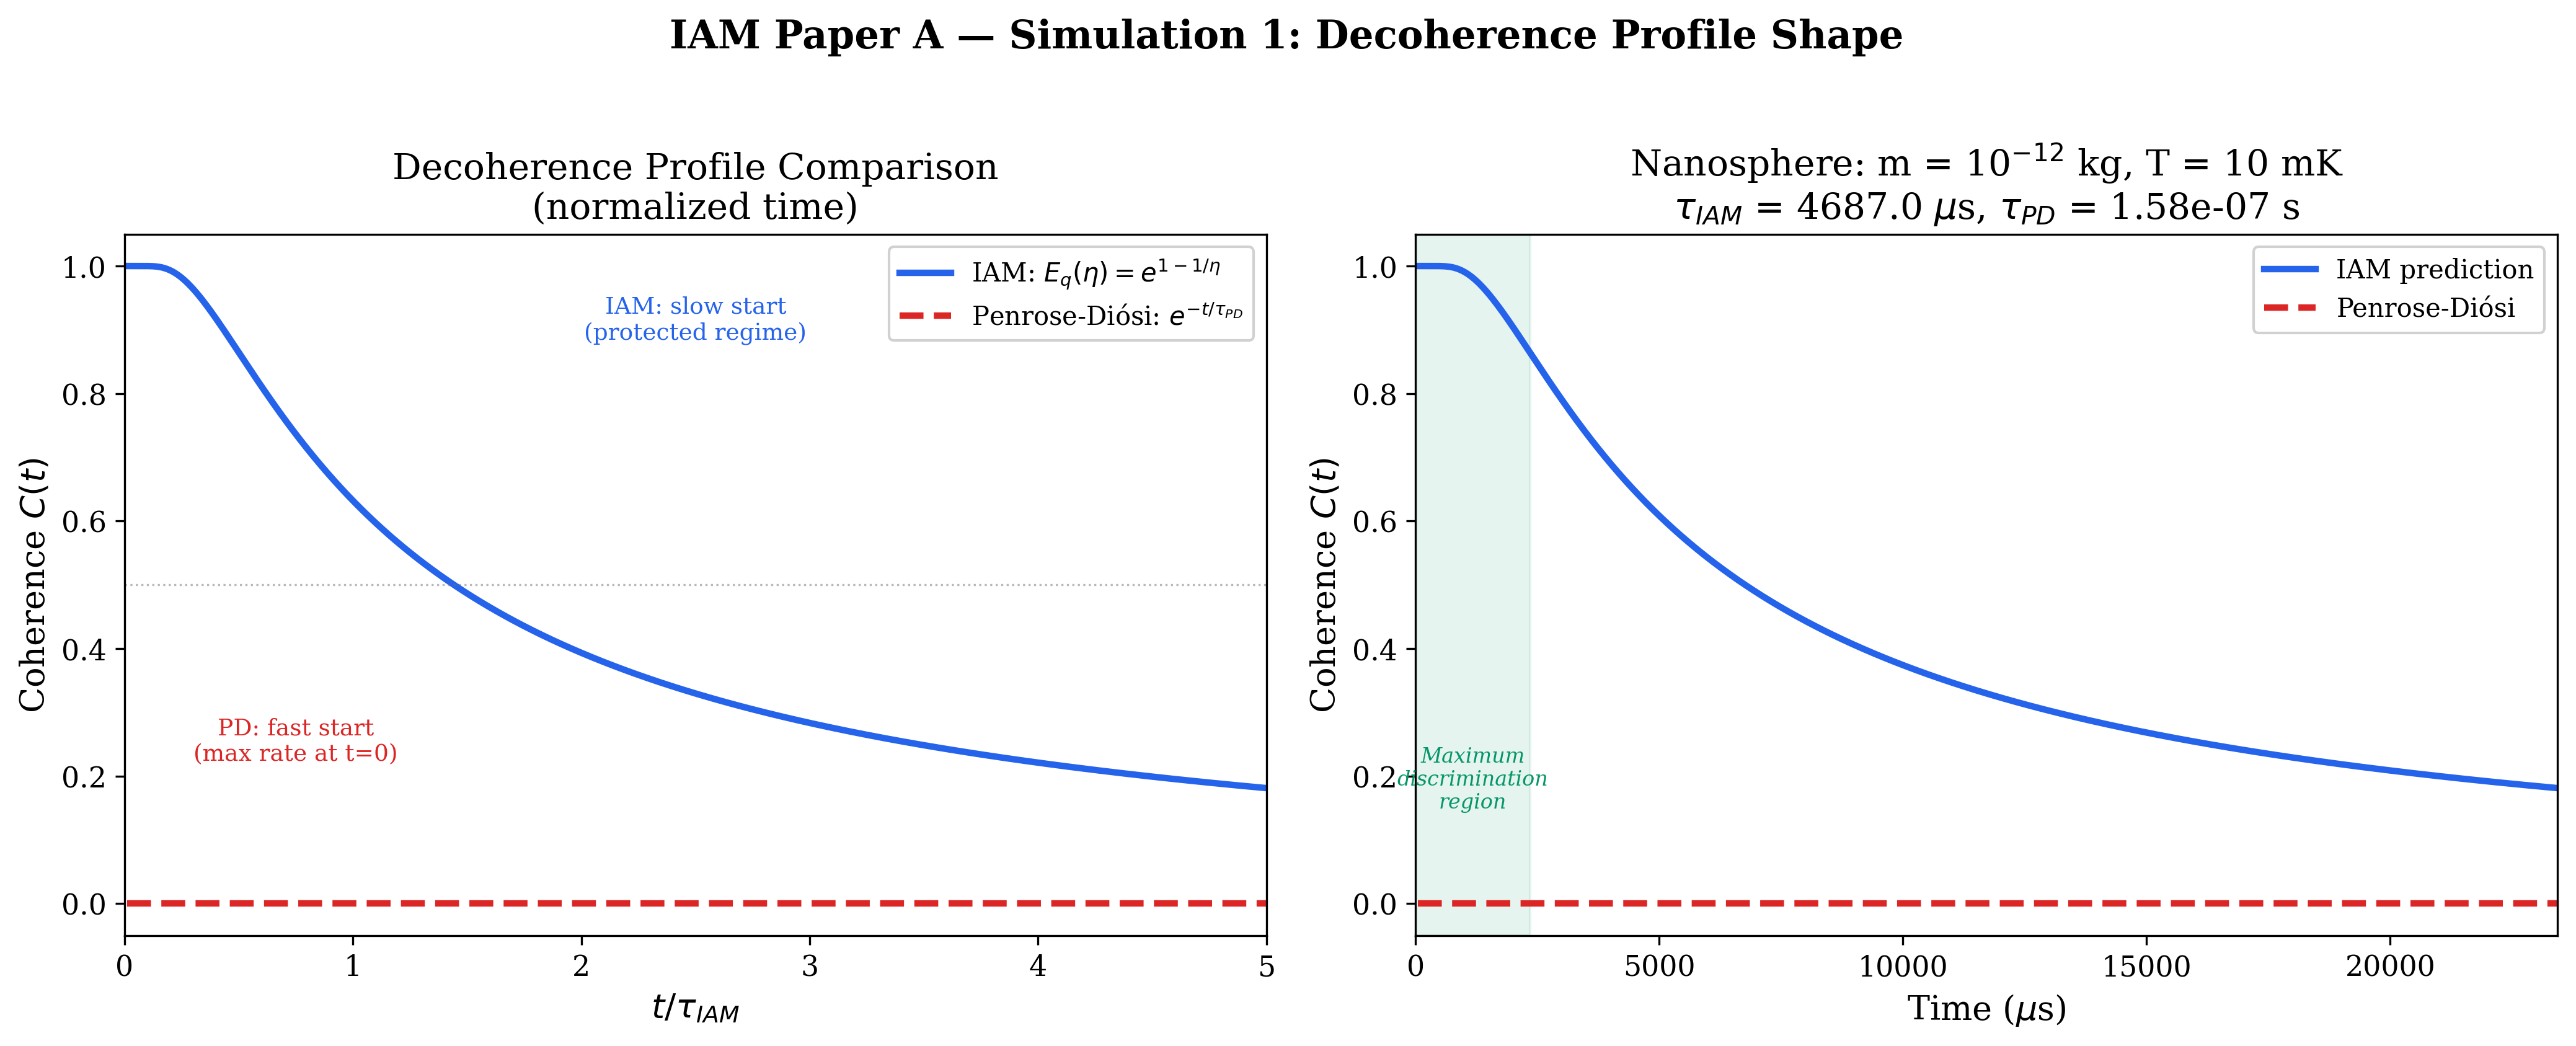
\includegraphics[width=0.92\textwidth]{fig1_decoherence_profiles.png}
\caption{Decoherence profile comparison for a $10^{-12}$~kg nanosphere
at 10~mK. \textbf{Left:} Normalized time. \IAM{} (blue) shows zero rate
at $t = 0$ (protected regime); Penrose--Di\'{o}si (red dashed) shows
maximum rate at $t = 0$. \textbf{Right:} Physical timescale in $\mu$s.
Green shading marks the maximum discrimination region ($t < 0.5\,\tauIAM$).}
\label{fig:profiles}
\end{figure}

Figure~\ref{fig:rate} shows the decoherence rate profiles, making the
qualitative difference at early times explicit.

\begin{figure}[H]
\centering
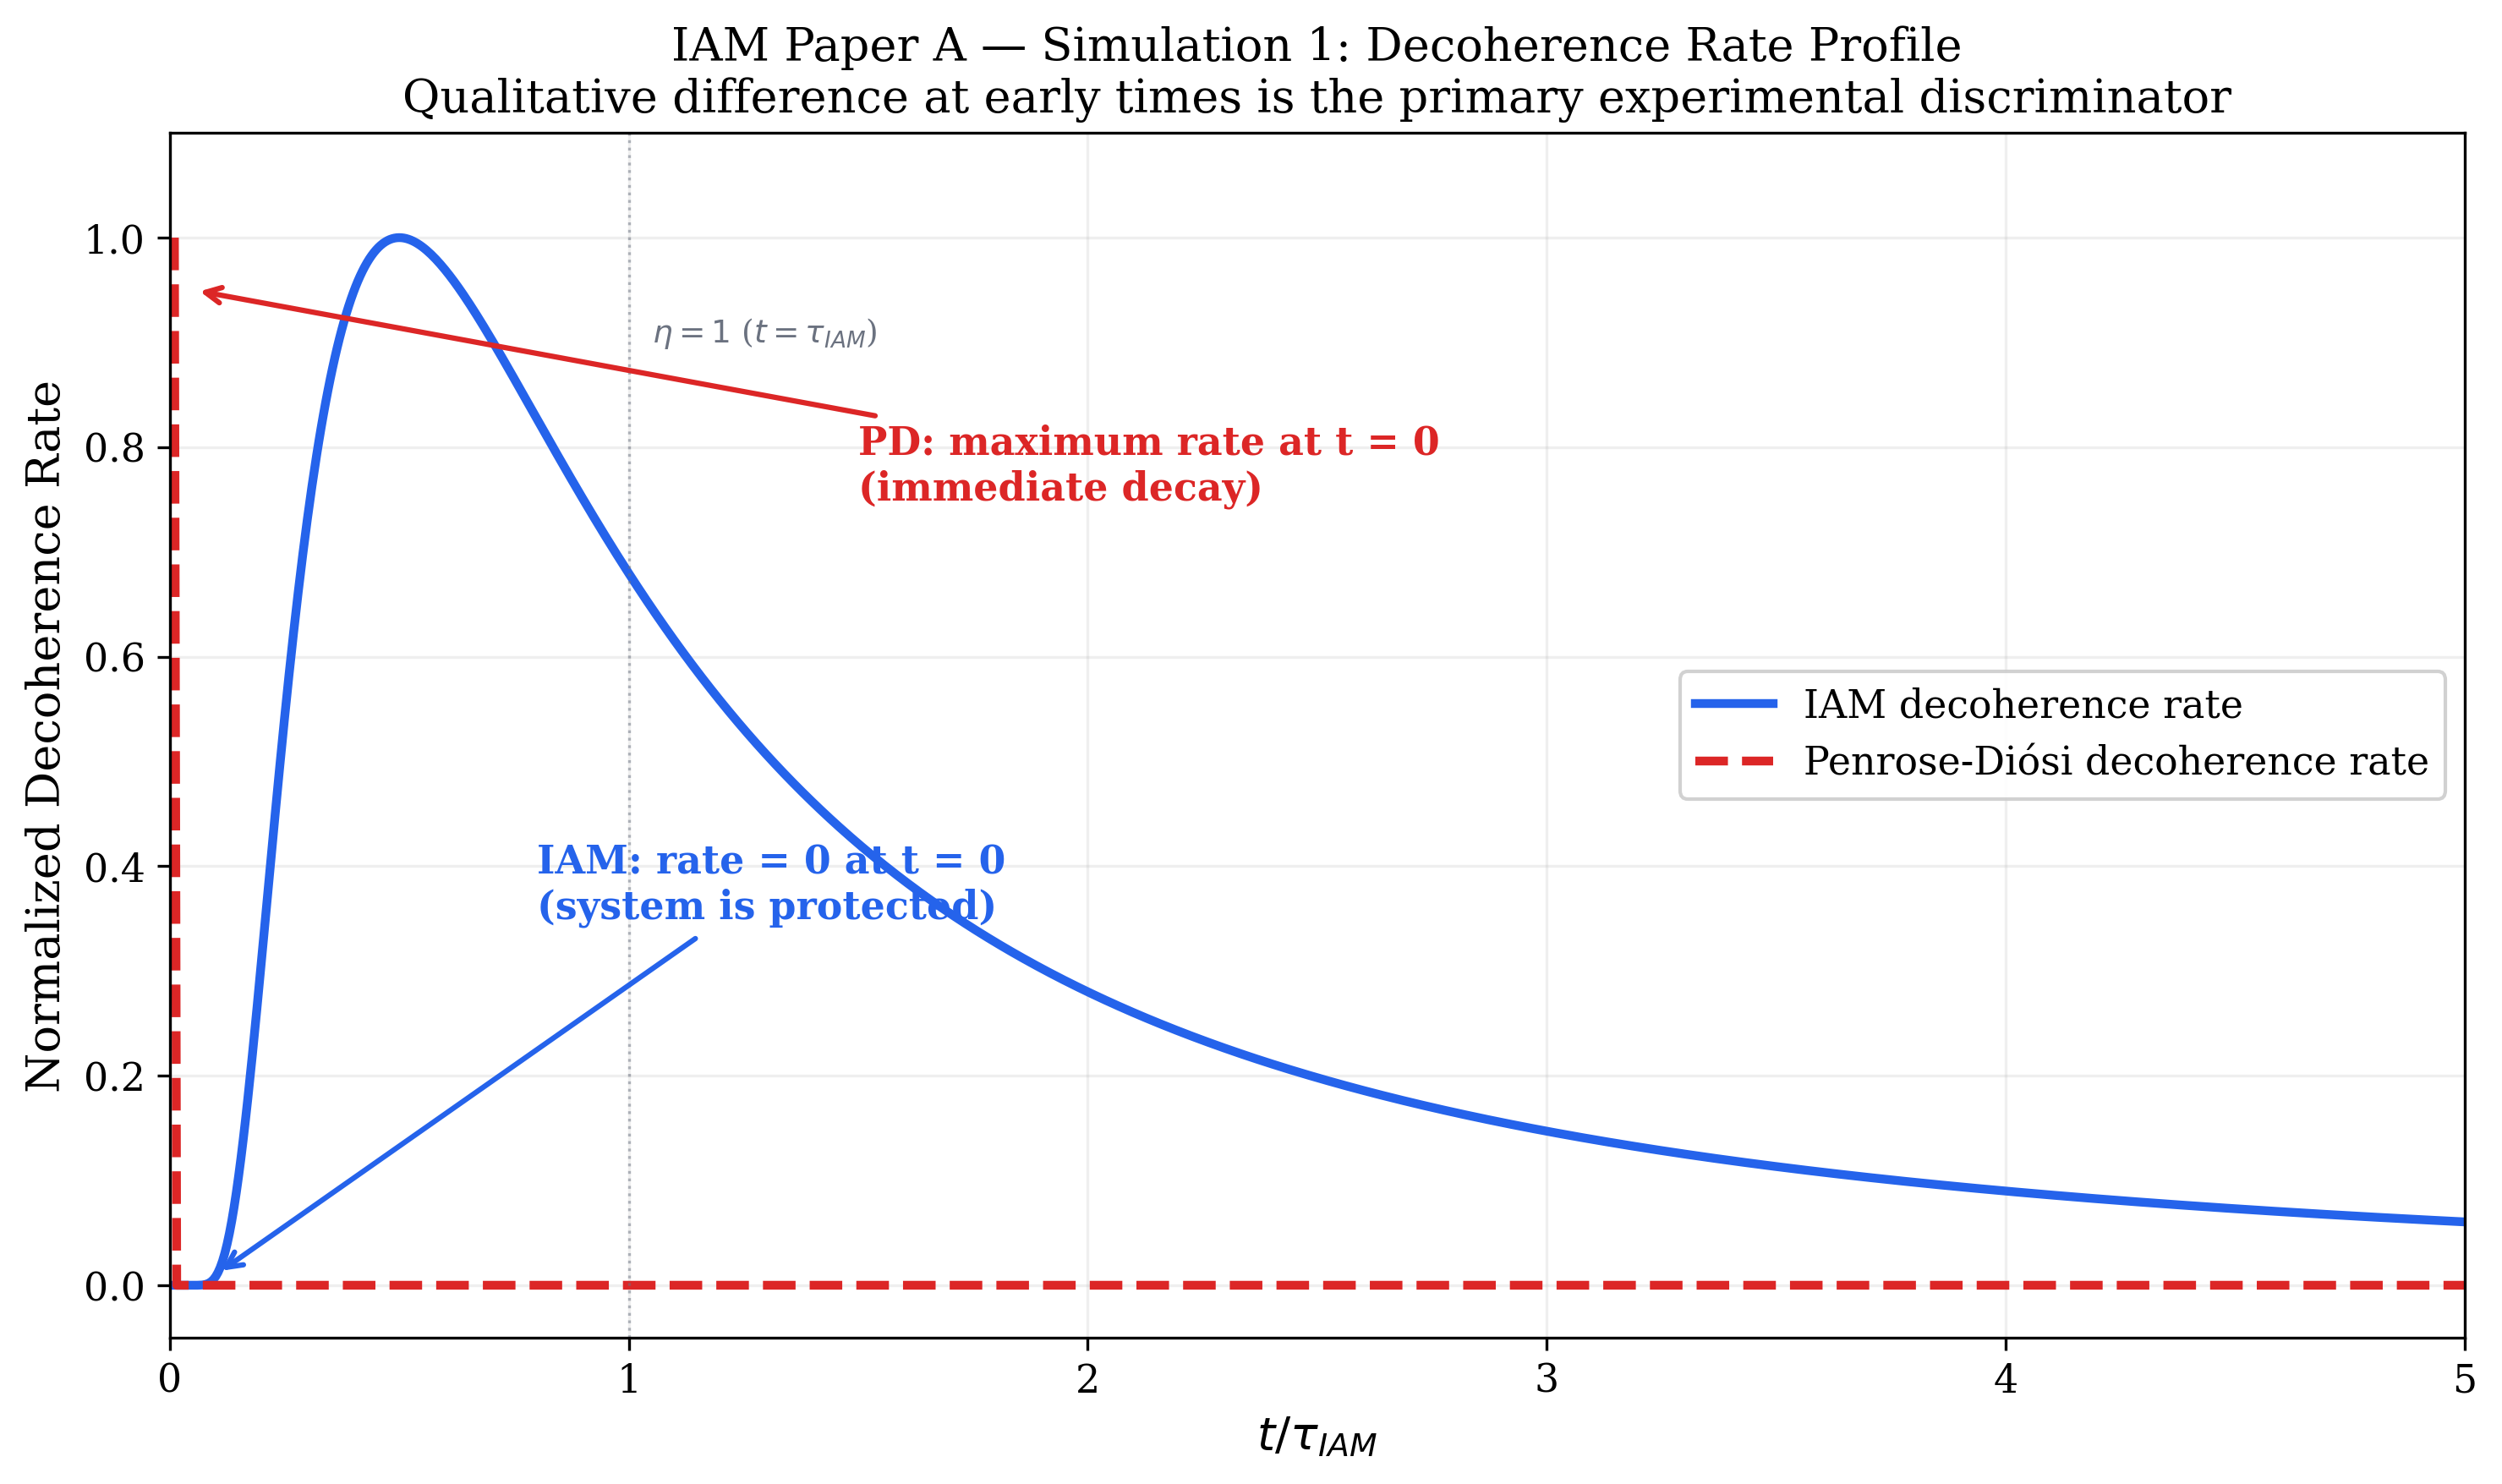
\includegraphics[width=0.80\textwidth]{fig4_decoherence_rate.png}
\caption{Normalized decoherence rate $-dC/dt$ for IAM (blue) and
Penrose--Di\'{o}si (red dashed). \IAM{} rate is zero at $t = 0$ and
peaks near $\eta \approx 0.5$. Penrose--Di\'{o}si rate is maximum at
$t = 0$. This qualitative difference is the primary experimental
discriminator, accessible at early times without high-precision
measurements.}
\label{fig:rate}
\end{figure}

% ============================================================
\section{Quantitative Predictions}
% ============================================================

\subsection{Timescales Across Mass Scales}

Figure~\ref{fig:tau_mass} shows $\tauIAM$ versus mass from trapped ions
to dust grains at five temperatures, compared against Penrose--Di\'{o}si.
The mesoscopic frontier ($10^{-15}$--$10^{-10}$~kg) is where predictions
become testable with current experimental reach ($\sim$100~$\mu$s).

\begin{figure}[H]
\centering
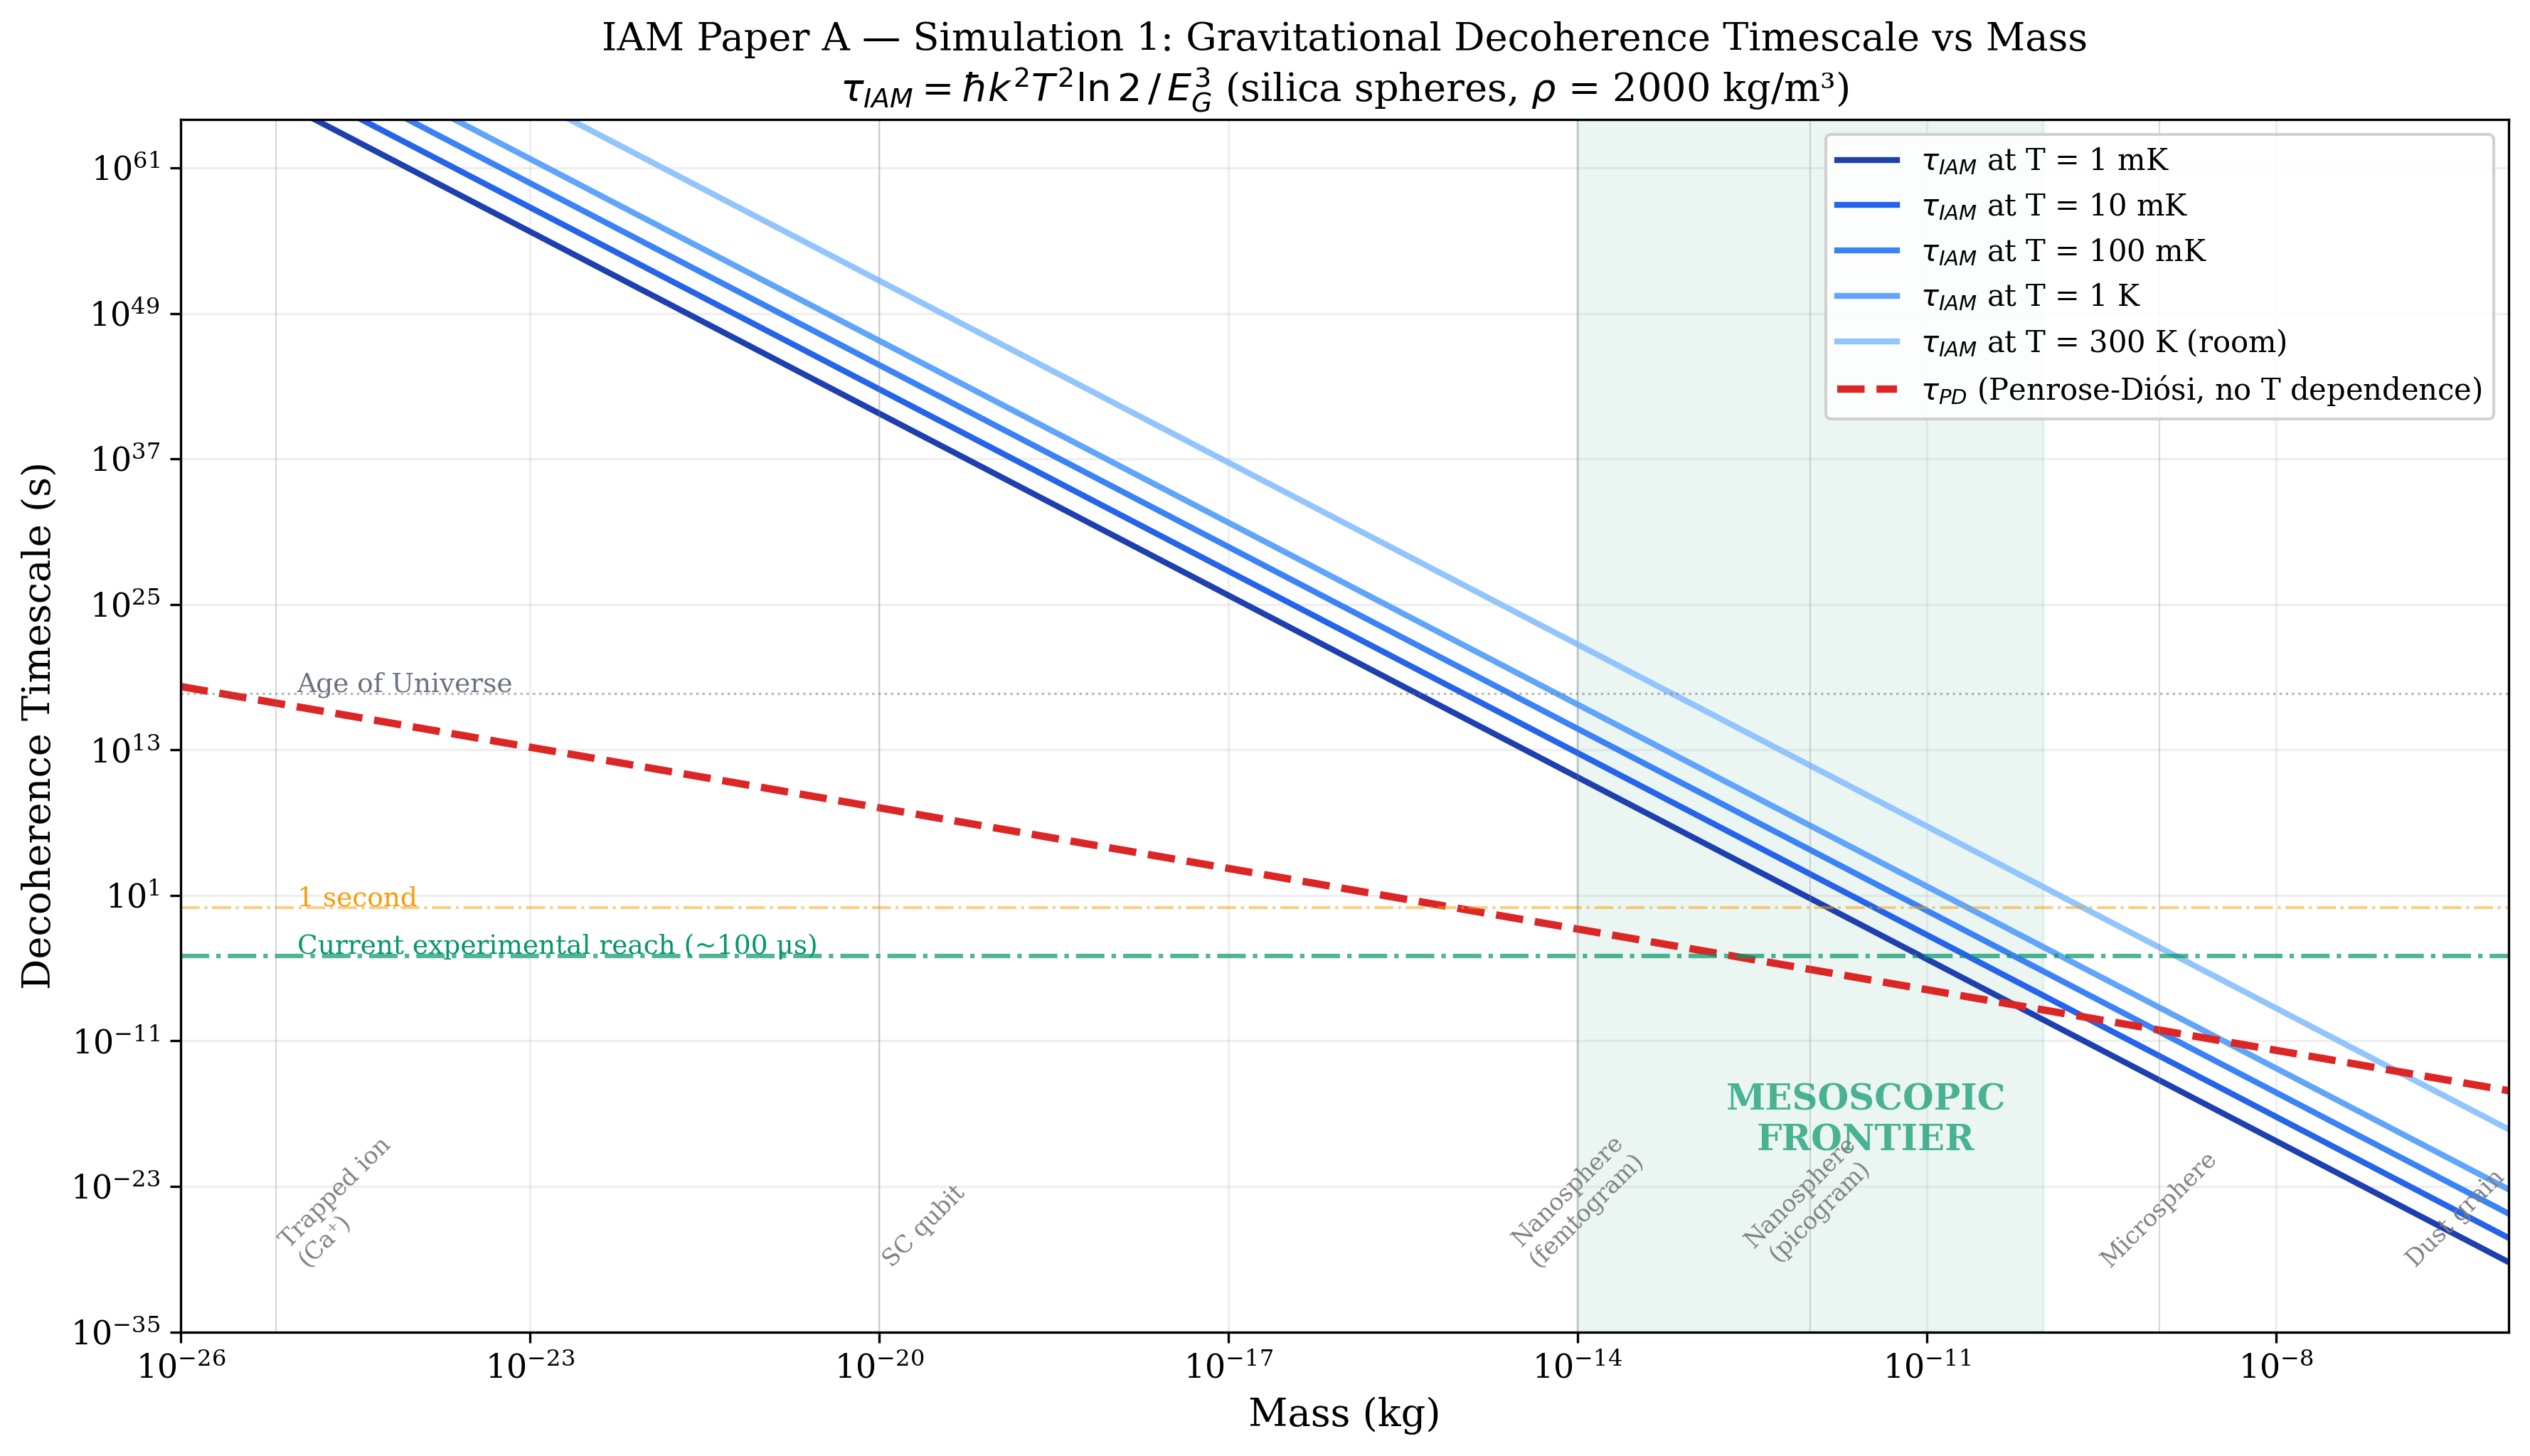
\includegraphics[width=0.90\textwidth]{fig2_tau_vs_mass.png}
\caption{Gravitational decoherence timescale $\tauIAM$ versus mass for
silica spheres ($\rho = 2000$~kg/m$^3$) at five temperatures (1~mK to
300~K), compared against Penrose--Di\'{o}si (red dashed, no temperature
dependence). The green shaded mesoscopic frontier marks the experimentally
accessible regime. The $T^2$ temperature dependence of \IAM{} separates
the colored curves; Penrose--Di\'{o}si produces a single curve.}
\label{fig:tau_mass}
\end{figure}

\subsection{Temperature Dependence: The Key Discriminator}

Figure~\ref{fig:temperature} shows $\tauIAM \propto T^2$ for a fixed
nanosphere mass. Running the same experiment at 10, 20, and 40~mK
produces a factor of 4 and 16 increase in $\tauIAM$ respectively.
Penrose--Di\'{o}si predicts no change. This is the single cleanest test.

\begin{figure}[H]
\centering
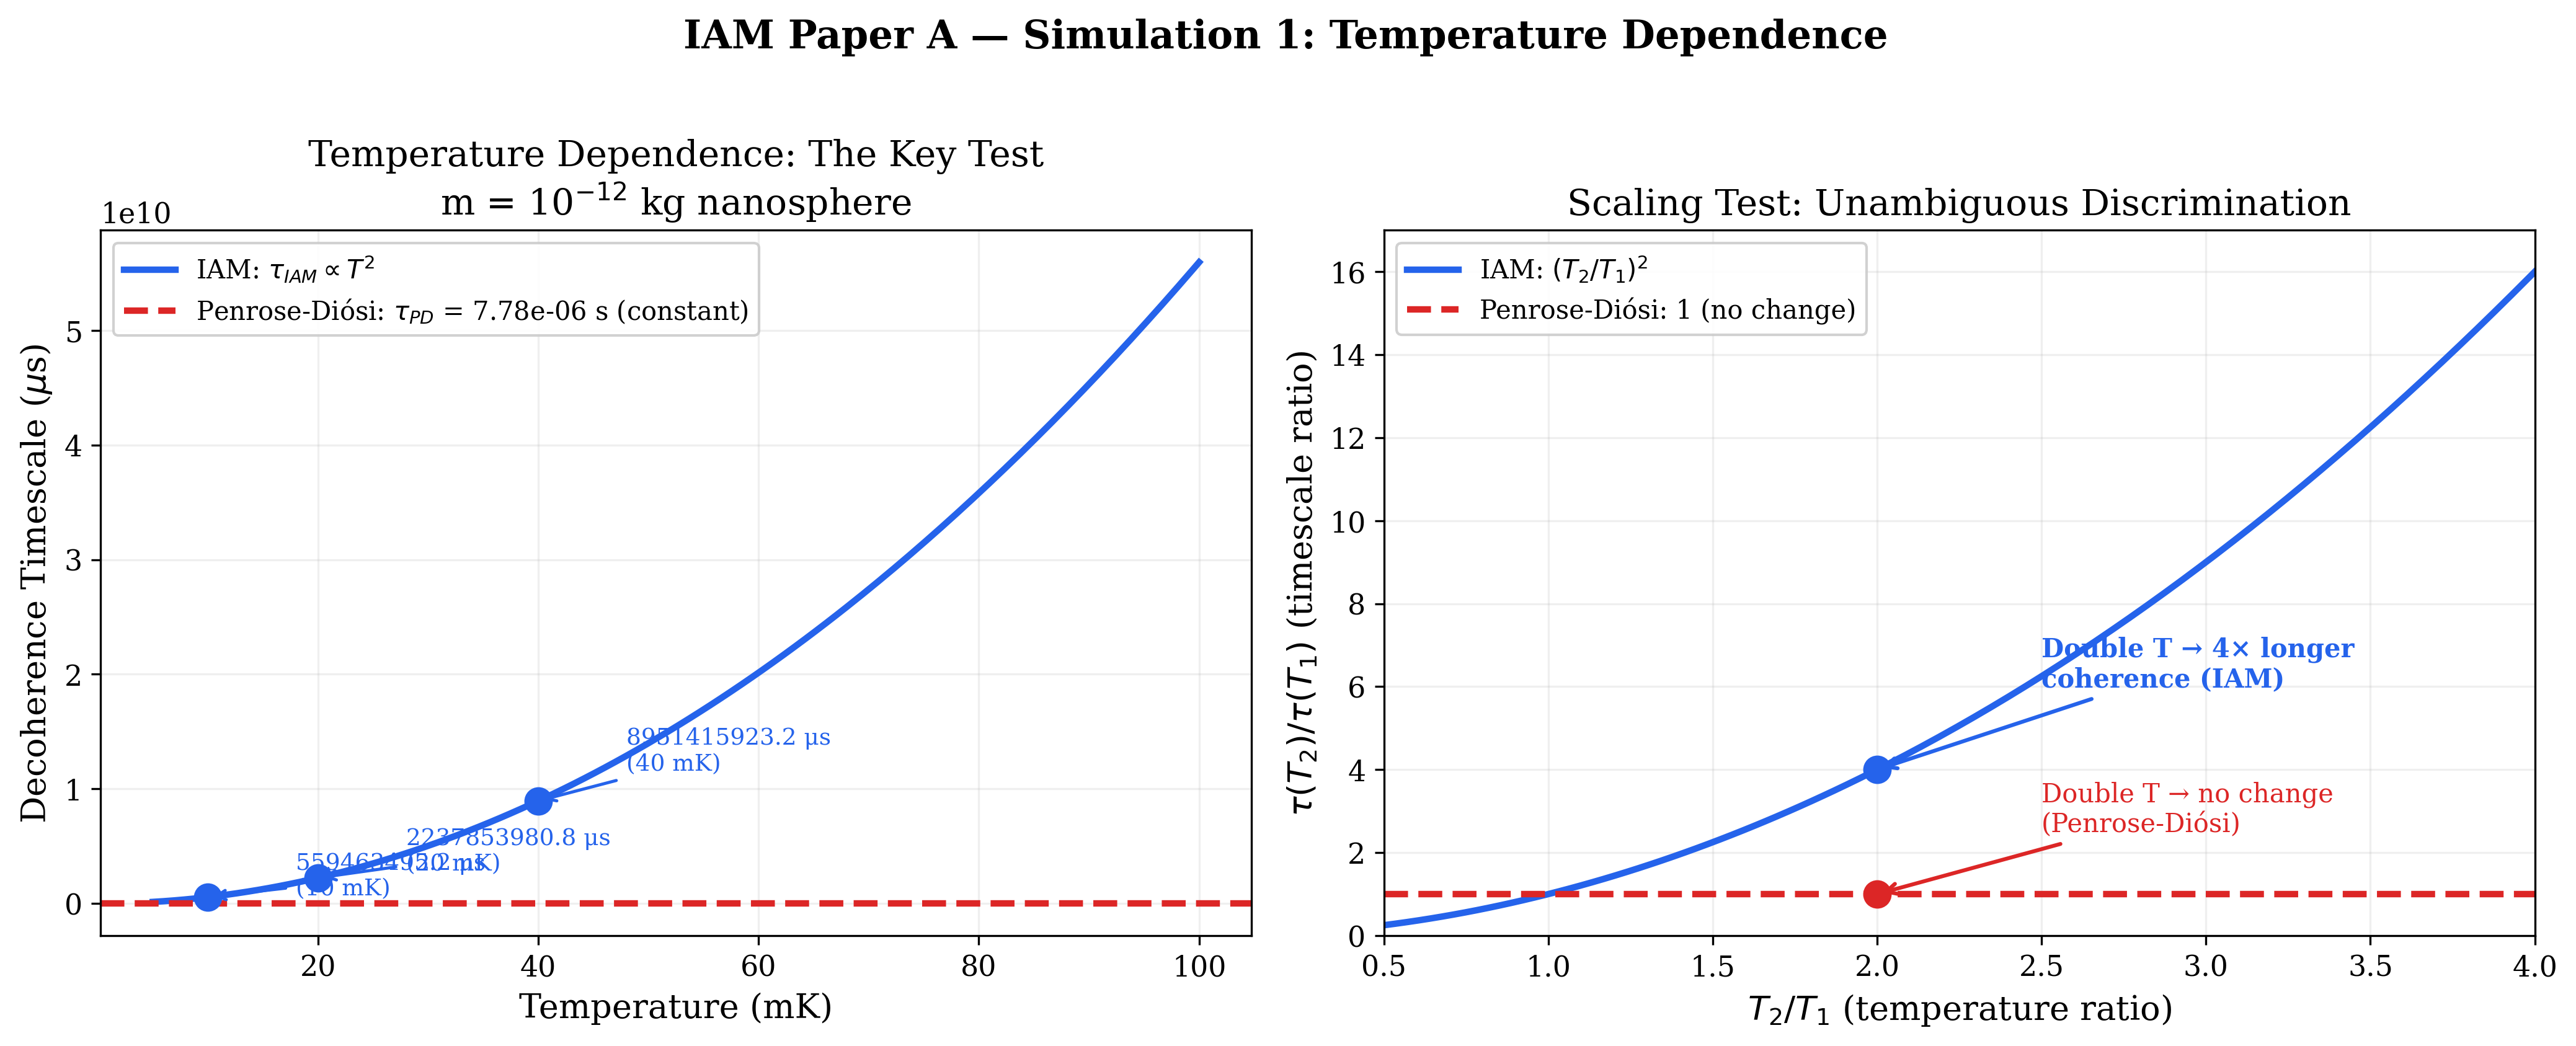
\includegraphics[width=0.92\textwidth]{fig3_temperature_dependence.png}
\caption{\textbf{Left:} $\tauIAM$ versus temperature for a $10^{-12}$~kg
nanosphere. \IAM{} (blue): $\tau \propto T^2$, with specific values at
10, 20, and 40~mK marked. Penrose--Di\'{o}si (red dashed): no temperature
dependence. \textbf{Right:} Timescale ratio $\tau(T_2)/\tau(T_1)$ versus
temperature ratio. \IAM{} scales as $(T_2/T_1)^2$; Penrose--Di\'{o}si
gives ratio $= 1$ always. Doubling the temperature produces a 4$\times$
longer coherence time under \IAM{} --- unambiguous discrimination.}
\label{fig:temperature}
\end{figure}

\subsection{Mass Scaling in the Mesoscopic Regime}

Figure~\ref{fig:mass_scaling} shows $\tauIAM \propto m^{-6}$ versus
Penrose--Di\'{o}si $\tauPD \propto m^{-5/3}$ in the mesoscopic regime.
The crossover occurs near $m \approx 2.3 \times 10^{-10}$~kg. Below the
crossover, \IAM{} predicts slower decoherence (thermal bath absorbs events);
above it, \IAM{} predicts faster decoherence (cumulative ramp dominates).
Measuring $\tau$ at 3--4 bead masses spanning one order of magnitude
discriminates between log slopes of $-6$ and $-5/3$ at $> 5\sigma$ with
10\% precision.

\begin{figure}[H]
\centering
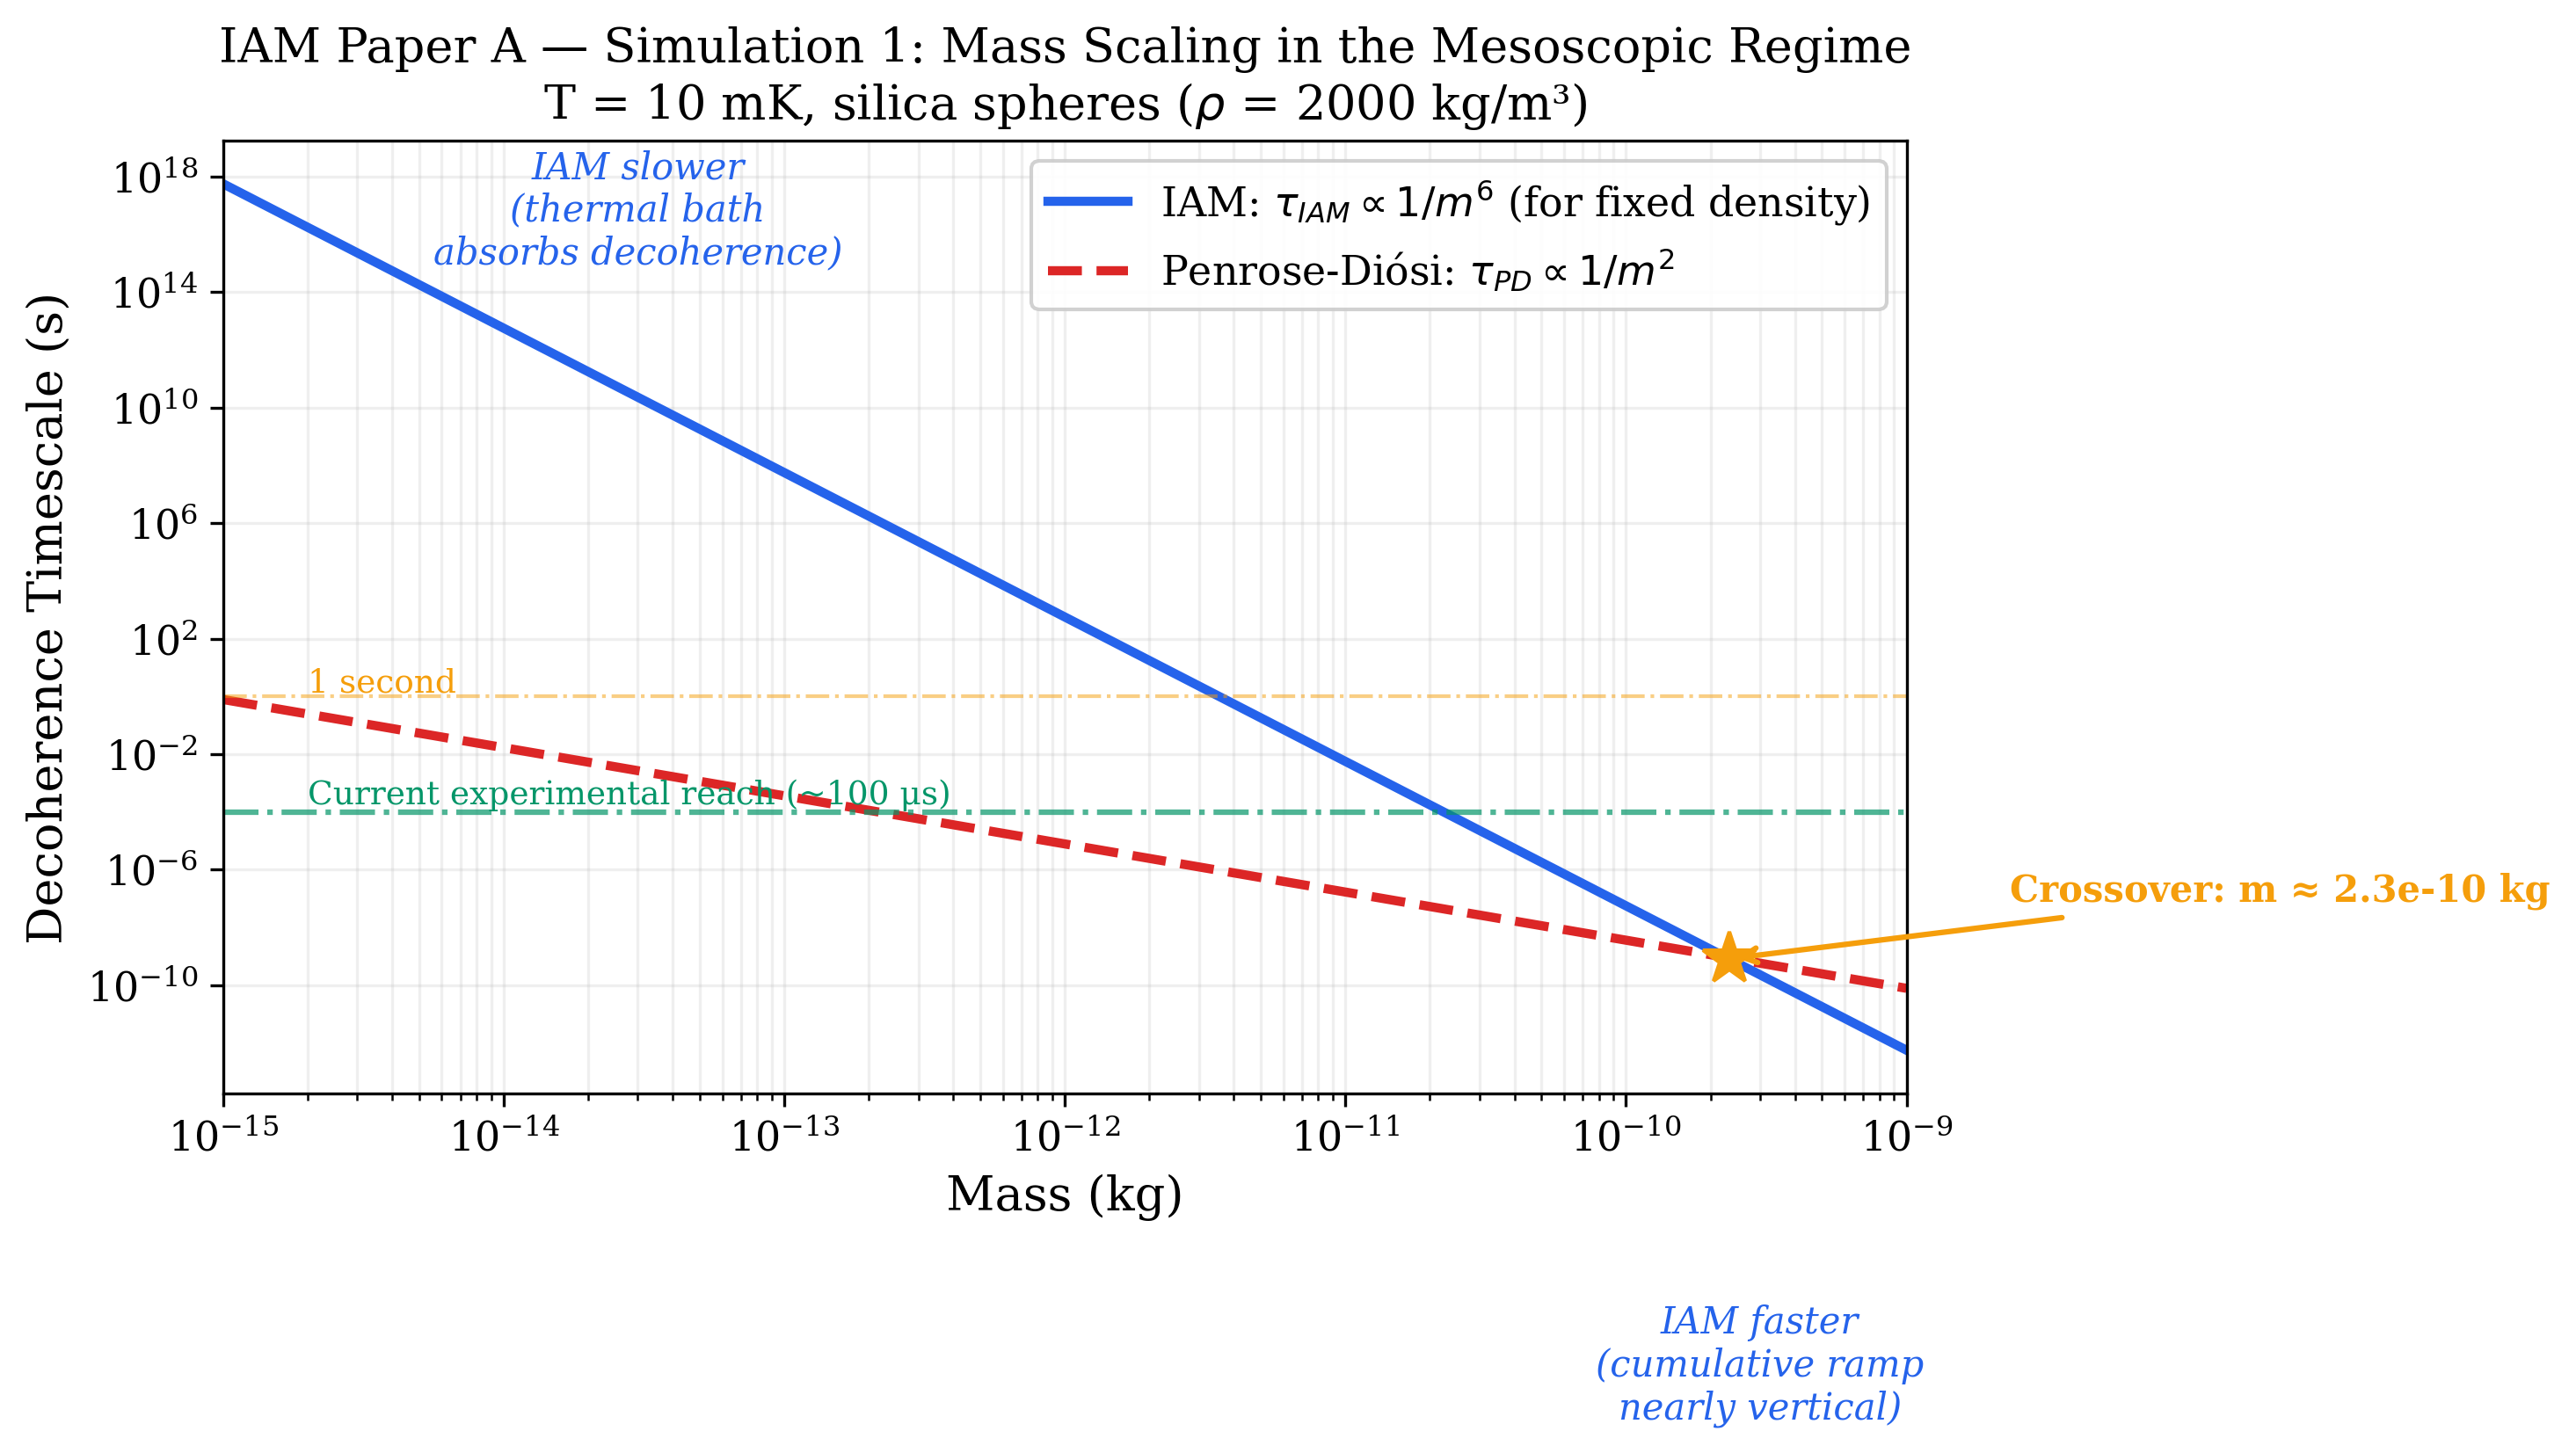
\includegraphics[width=0.80\textwidth]{fig5_mass_scaling.png}
\caption{Decoherence timescale versus mass in the mesoscopic regime at
$T = 10$~mK. \IAM{} (blue): $\tau \propto m^{-6}$. Penrose--Di\'{o}si
(red dashed): $\tau \propto m^{-5/3}$. Crossover at $m \approx
2.3 \times 10^{-10}$~kg (gold star). The difference in power law exponent
($\Delta\alpha = 4.33$) is measurable at $5\sigma$ with 3--4 bead masses.}
\label{fig:mass_scaling}
\end{figure}

\subsection{Landauer Heating Rate}

Each decoherence event produces irreversible information at Landauer cost
$\kB T \ln 2$. The dissipated power and phonon excitation rate are:
\begin{equation}
    P_{\rm IAM} = \frac{\EG^3}{\hbar \kB T}, \qquad
    \frac{dn}{dt} = \frac{\EG^3}{\hbar^2 \kB T \omega_0}.
    \label{eq:heating}
\end{equation}
Critically, $P_{\rm IAM} \propto 1/T$ --- colder systems dissipate more
power per event. This is the inverse of environmental heating
($P_{\rm env} \propto T$) and provides an unambiguous discriminator.

% ============================================================
\section{Modified Lindblad Dynamics}
% ============================================================

\subsection{Time-Dependent Lindblad Rate}

The \IAM{} $E_q$ ramp implies a time-dependent Lindblad decoherence rate:
\begin{equation}
    \Gamma_{\rm IAM}(t) = \frac{dE_q}{dt} \cdot \frac{1}{\tauIAM}
    = \frac{1}{\eta^2} \exp\!\left(1 - \frac{1}{\eta}\right),
    \quad \eta = t/\tauIAM.
    \label{eq:gamma_iam}
\end{equation}
The density matrix evolves under:
\begin{equation}
    \frac{d\rho}{d\eta} = \Gamma(\eta)\left(L\rho L^\dagger
    - \tfrac{1}{2}\{L^\dagger L,\, \rho\}\right),
    \label{eq:lindblad}
\end{equation}
where the collapse operator $L \propto \hat{x}$ (position) implements
gravitational dephasing: spatial coherence decays while energy (phonon
populations) is conserved.

\subsection{Quantum State Evolution}

Figure~\ref{fig:lindblad} shows the four-panel quantum state evolution for
a $10^{-12}$~kg nanosphere in an initial coherent state $|\alpha = 2\rangle$
at 10~mK, simulated via 4th-order Runge--Kutta in the interaction picture.

\begin{figure}[H]
\centering
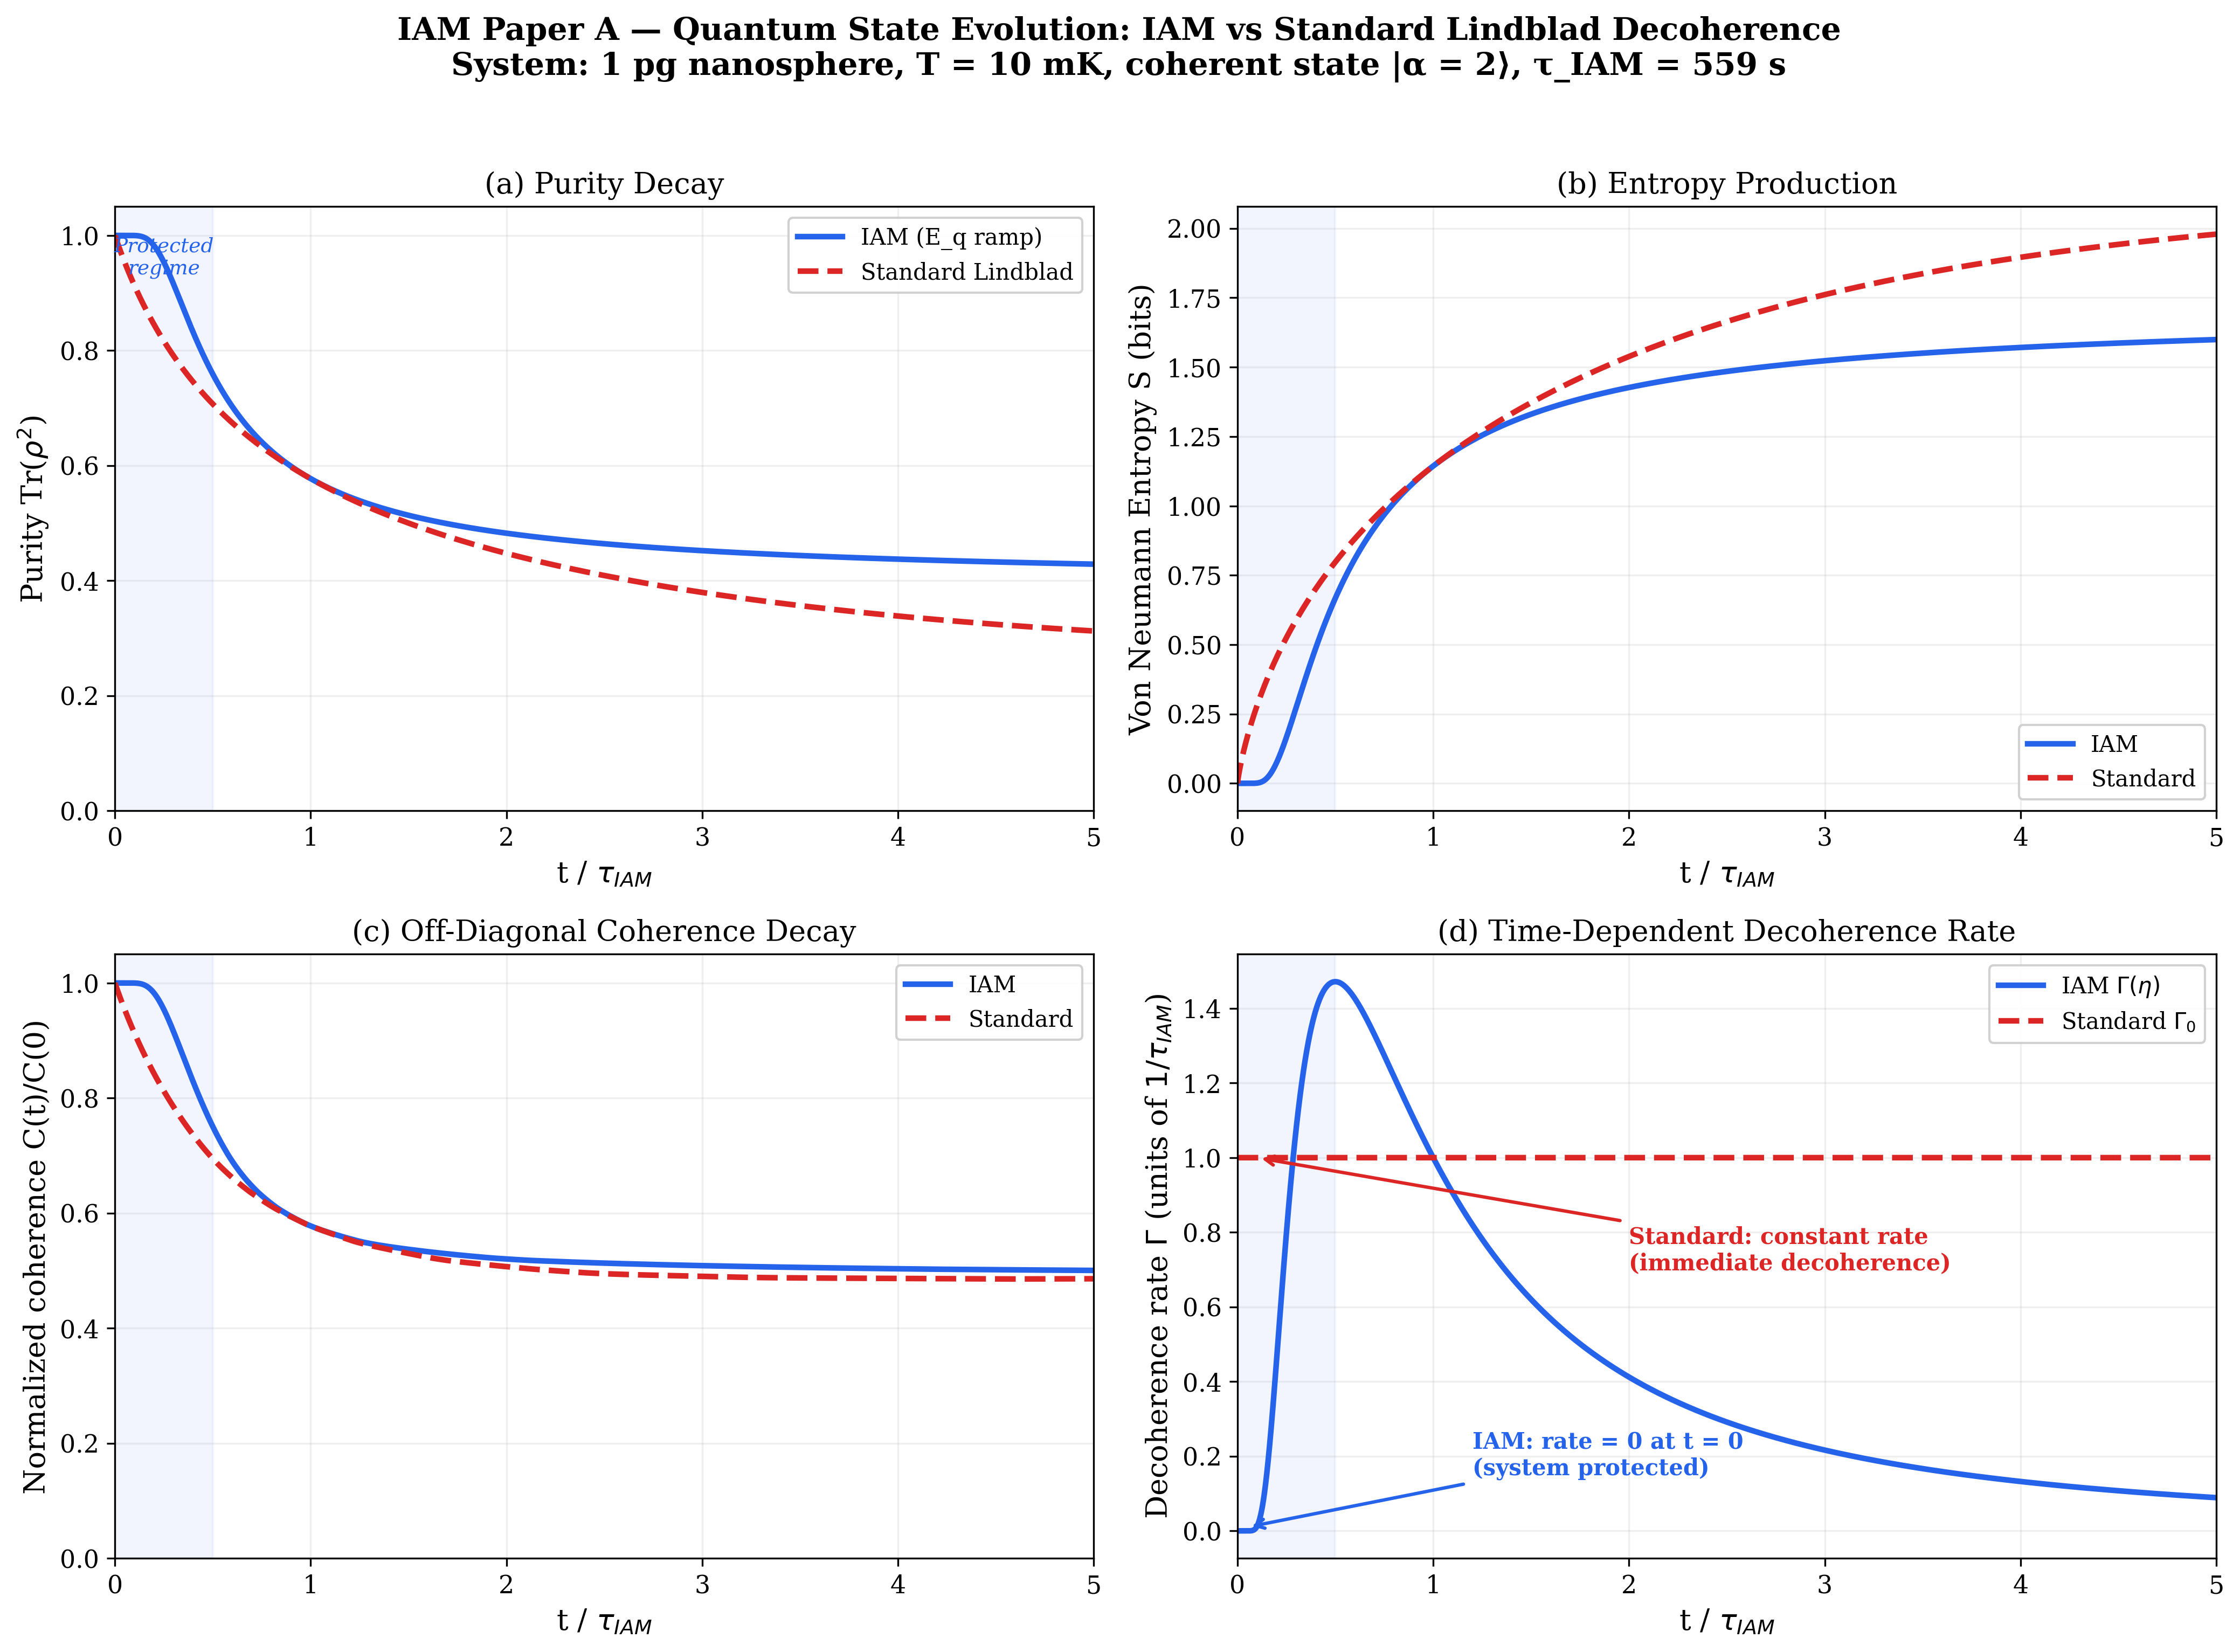
\includegraphics[width=0.95\textwidth]{fig10_lindblad_evolution.png}
\caption{Quantum state evolution under \IAM{} (blue) versus standard
Lindblad (red dashed) decoherence. \textbf{(a)} Purity Tr($\rho^2$): \IAM{}
maintains higher purity in the protected regime ($\eta < 0.5$, blue shading).
\textbf{(b)} Von Neumann entropy production: delayed onset under \IAM.
\textbf{(c)} Off-diagonal coherence normalized to initial value: \IAM{}
preserves coherence longer at early times.
\textbf{(d)} Time-dependent decoherence rate: \IAM{} rate is zero at
$t = 0$ and peaks near $\eta \approx 0.23$; standard rate is constant.
System: $10^{-12}$~kg nanosphere, $T = 10$~mK, $|\alpha = 2\rangle$.}
\label{fig:lindblad}
\end{figure}

\subsection{Density Matrix Snapshots}

Figure~\ref{fig:density_matrices} shows the Fock-space density matrix
$|\rho_{mn}|$ at five time steps for both \IAM{} and standard Lindblad
decoherence. The off-diagonal elements (quantum coherences) decay more
slowly under \IAM{} at early times, consistent with the protected regime
prediction.

\begin{figure}[H]
\centering
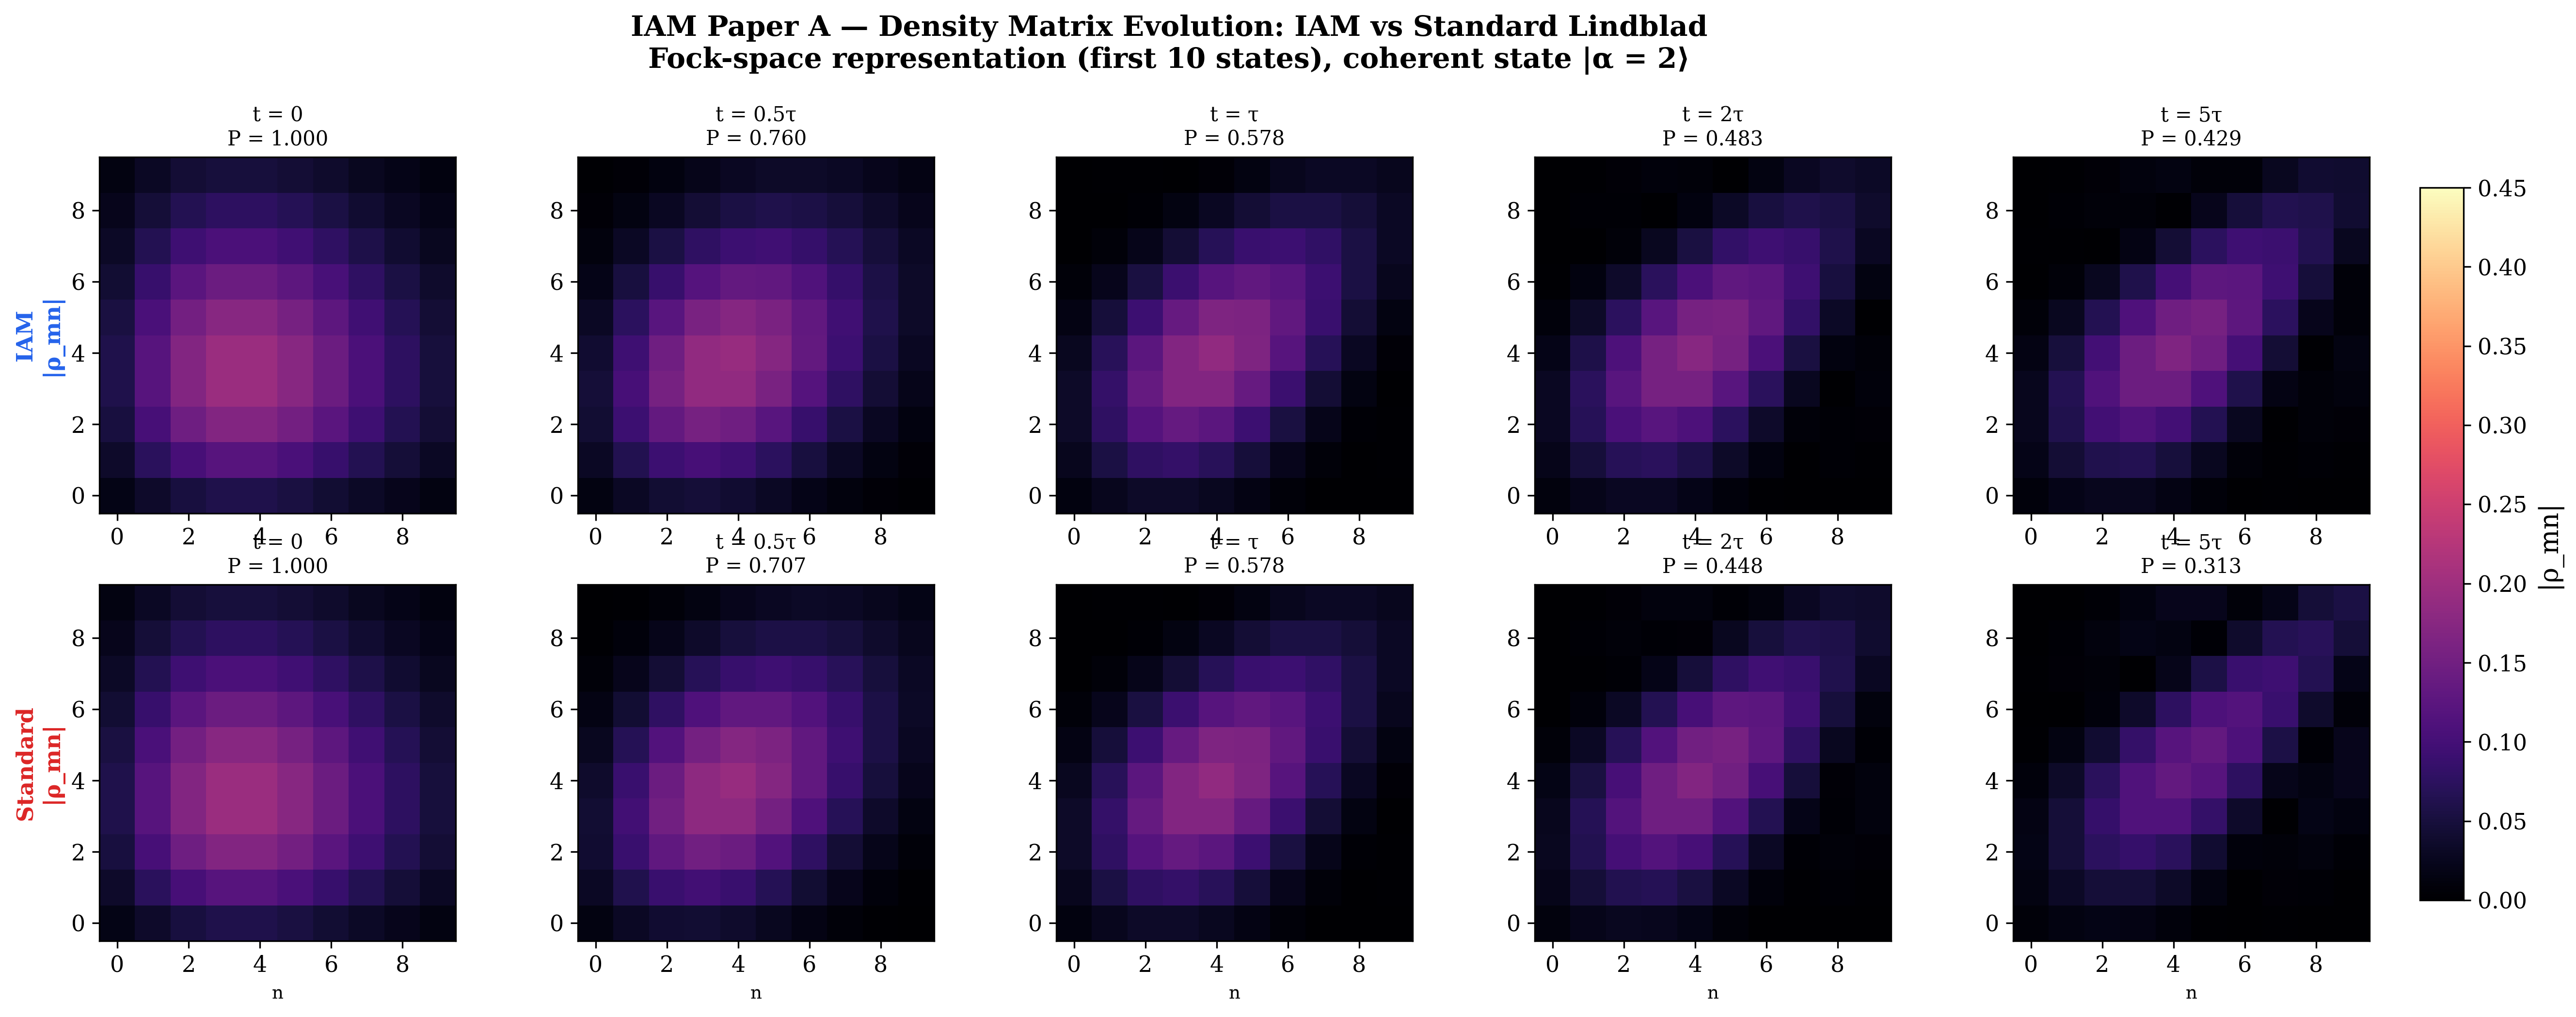
\includegraphics[width=0.95\textwidth]{fig11_density_matrices.png}
\caption{Density matrix snapshots $|\rho_{mn}|$ (first 10 Fock states)
at five time steps: $t = 0,\, 0.5\tau,\, \tau,\, 2\tau,\, 5\tau$.
\textbf{Top row:} \IAM{} decoherence. \textbf{Bottom row:} Standard
Lindblad decoherence. Purity $P$ shown for each snapshot. Off-diagonal
elements (quantum coherences) are preserved longer under \IAM{} at
early times. By $t = 5\tau$ both converge to approximately diagonal
(classical) states.}
\label{fig:density_matrices}
\end{figure}

\subsection{Information Thermodynamics}

Figure~\ref{fig:phonon_entropy} shows the phonon number decay, entropy
production rate, and purity difference between the two models. The purity
difference peaks near $\eta \approx 0.23$ --- the optimal measurement
time for discriminating \IAM{} from standard Lindblad decoherence.

\begin{figure}[H]
\centering
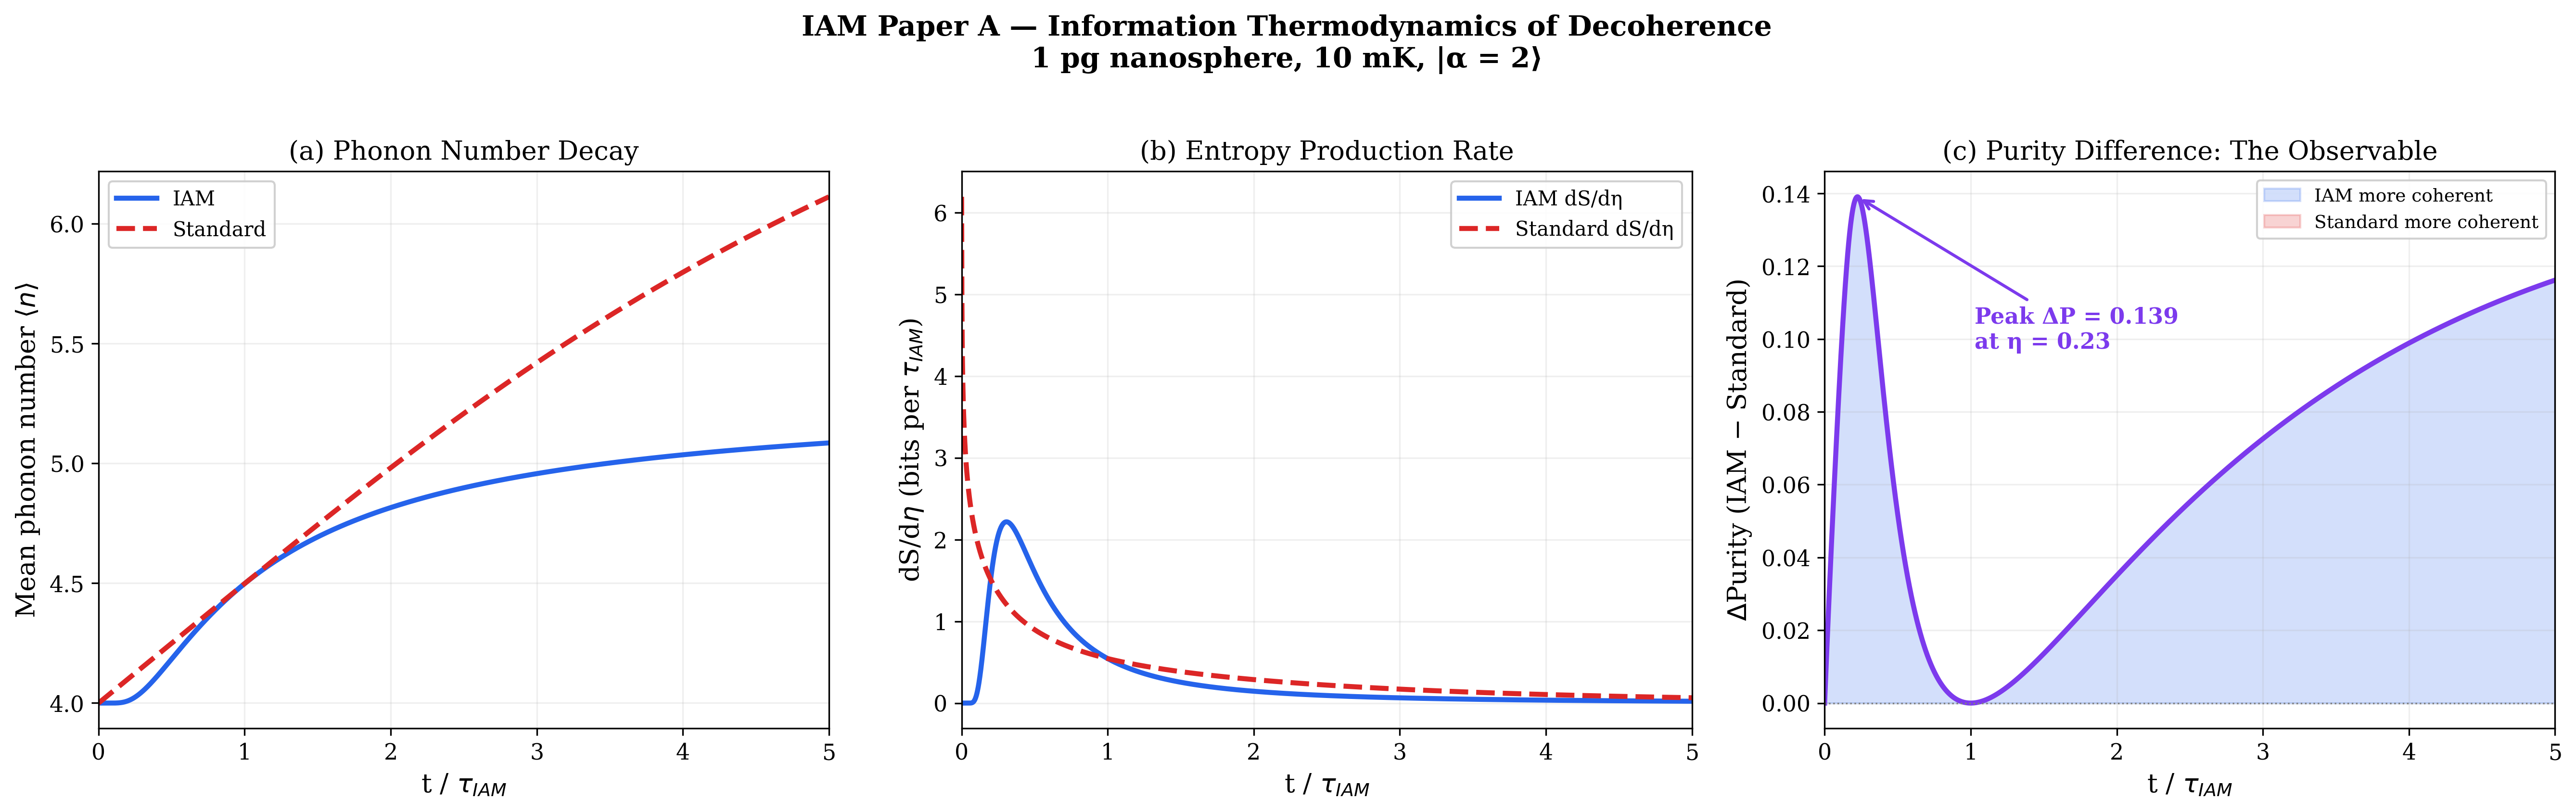
\includegraphics[width=0.95\textwidth]{fig12_phonon_entropy_purity.png}
\caption{\textbf{(a)} Mean phonon number $\langle n \rangle$ decay:
\IAM{} (blue) versus standard Lindblad (red). Phonon number is conserved
by position dephasing --- the decrease reflects state redistribution.
\textbf{(b)} Entropy production rate $dS/d\eta$: delayed onset under
\IAM{} reflects the protected regime.
\textbf{(c)} Purity difference $\Delta P = P_{\rm IAM} - P_{\rm std}$:
peaks at $\eta \approx 0.23$ ($\Delta P \approx 0.14$). This is the
observable experimental quantity and the optimal measurement time.}
\label{fig:phonon_entropy}
\end{figure}

% ============================================================
\section{Detection Forecasts}
% ============================================================

\subsection{Profile Shape Discrimination}

For an experiment measuring coherence $C(t)$ at $N = 50$ time points
with $\sigma_C = 2\%$ precision at $T = 10$~mK (Figure~\ref{fig:forecast_profile}):
\begin{align}
    3\sigma~\text{detection:} & \quad m > 3.7 \times 10^{-15}~\mathrm{kg}, \\
    5\sigma~\text{discovery:} & \quad m > 3.7 \times 10^{-15}~\mathrm{kg}.
\end{align}
Above $10^{-12}$~kg the SNR exceeds $100\sigma$. Even at 10\% precision,
$5\sigma$ discrimination is achieved above $\sim 10^{-13}$~kg.

\begin{figure}[H]
\centering
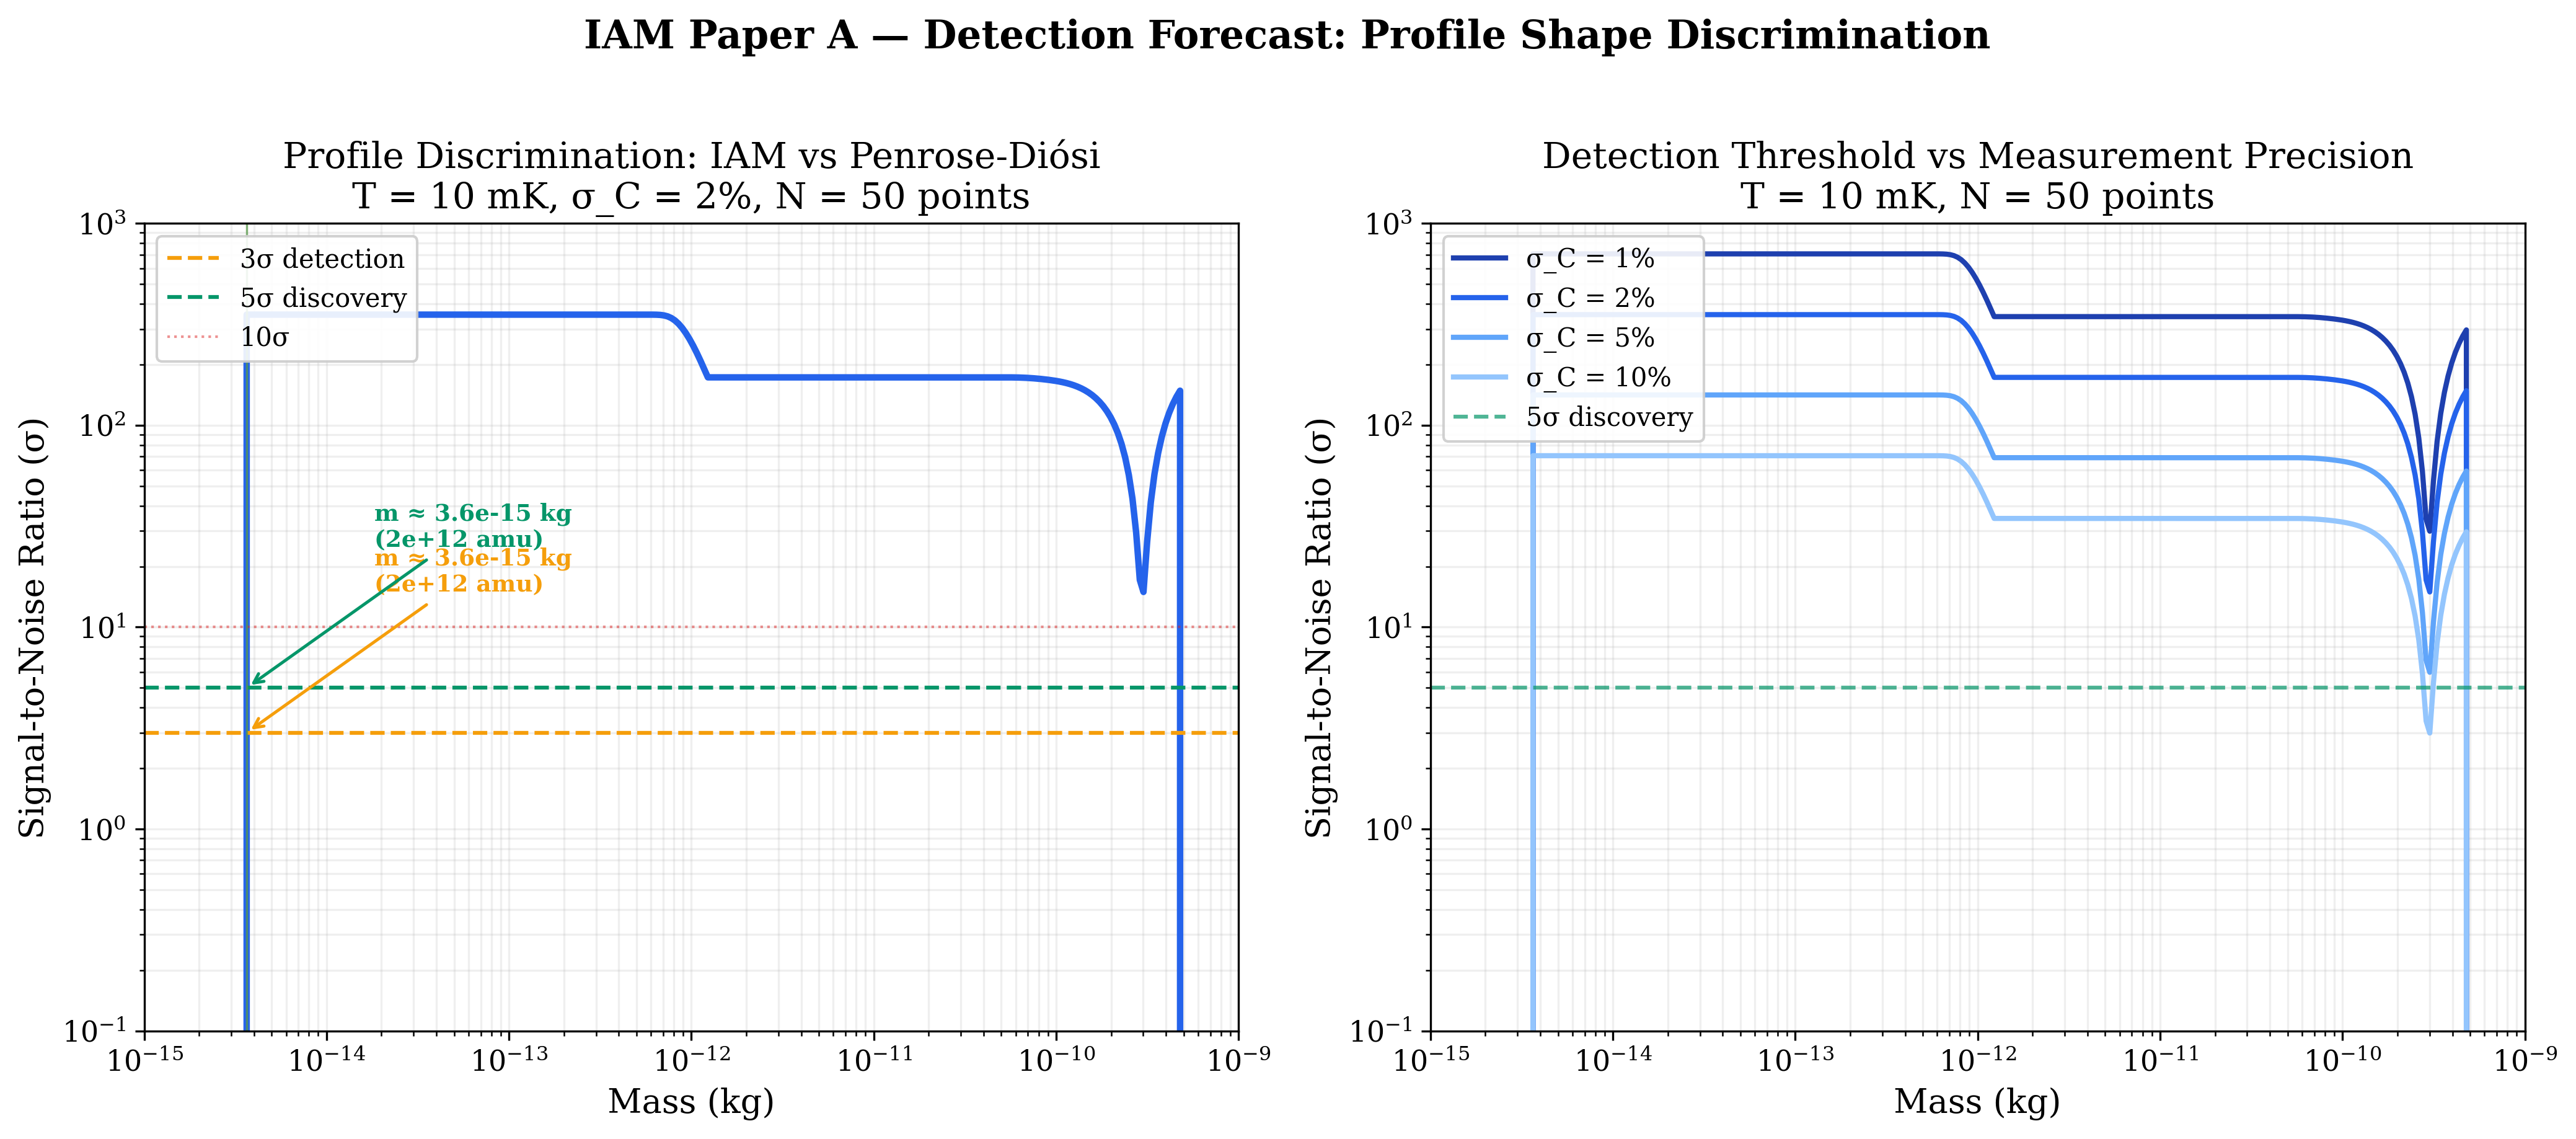
\includegraphics[width=0.92\textwidth]{fig6_detection_forecast_profile.png}
\caption{\textbf{Left:} SNR for profile shape discrimination versus mass
($T = 10$~mK, $\sigma_C = 2\%$, $N = 50$ points). $3\sigma$ (amber) and
$5\sigma$ (green) thresholds marked. Both crossed above
$3.7 \times 10^{-15}$~kg. \textbf{Right:} Detection threshold versus
measurement precision $\sigma_C$ from 1\% to 10\%. Even with 10\% precision,
$5\sigma$ discovery is achievable above $\sim 10^{-13}$~kg.}
\label{fig:forecast_profile}
\end{figure}

\subsection{Temperature and Mass Scaling Forecasts}

Figure~\ref{fig:forecast_scaling} shows the discrimination power of the
temperature scaling test (three temperatures at 10, 20, 40~mK) and mass
scaling test (four masses spanning one decade).

\begin{figure}[H]
\centering
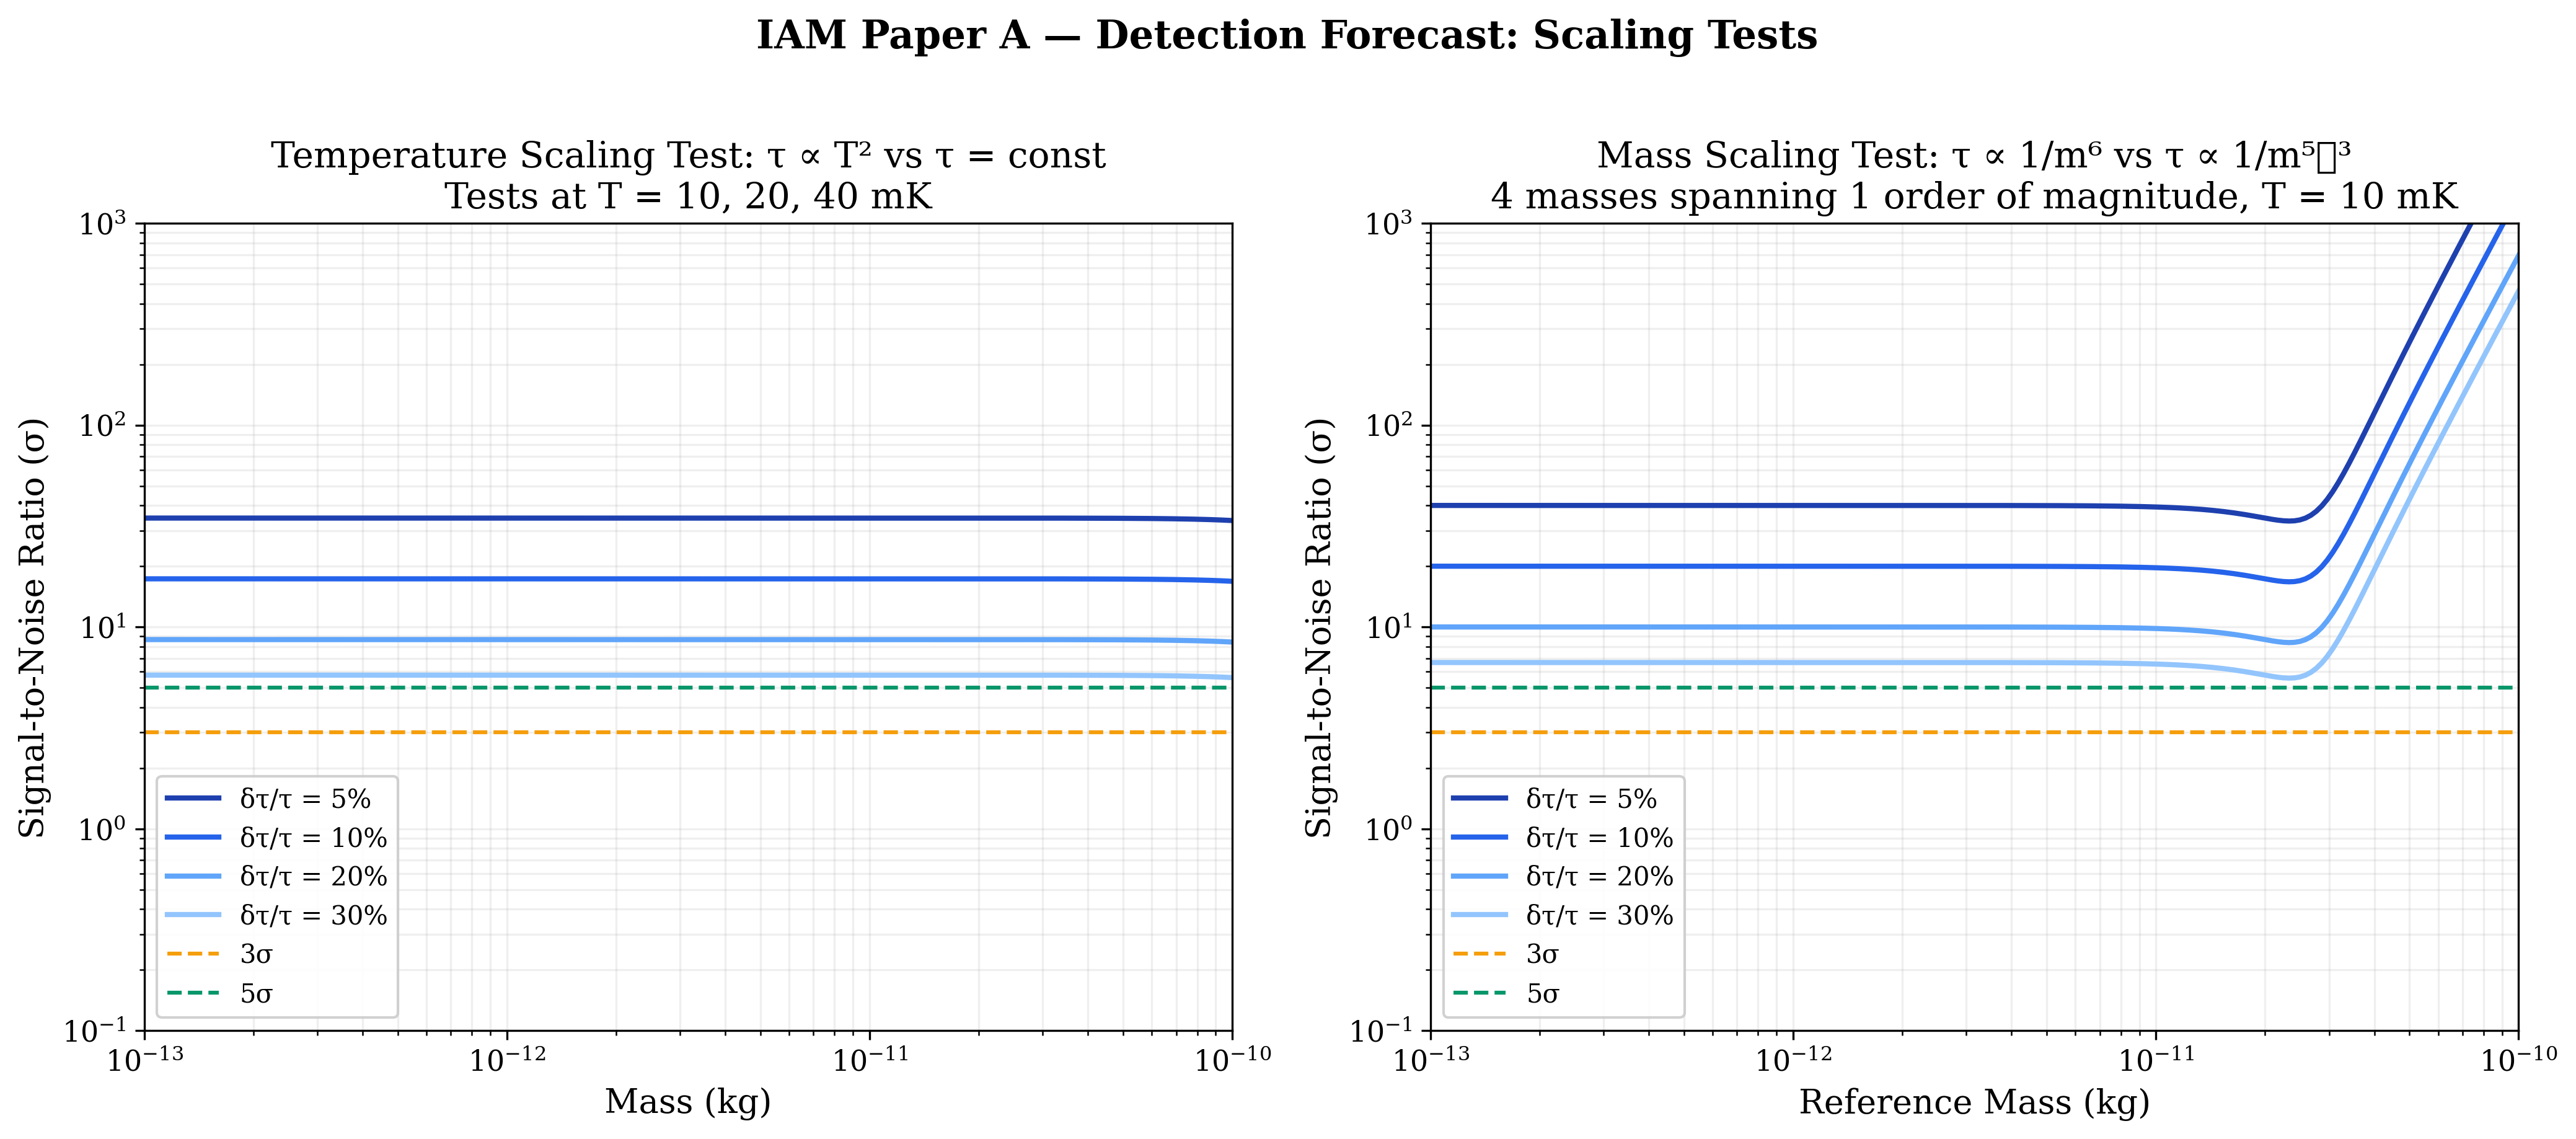
\includegraphics[width=0.92\textwidth]{fig7_detection_forecast_scaling.png}
\caption{\textbf{Left:} SNR for detecting $\tau \propto T^2$ versus
constant $\tau$ (Penrose--Di\'{o}si) from three temperature measurements.
$5\sigma$ discrimination achievable across the entire mesoscopic mass range
with 20\% precision on $\tau$. \textbf{Right:} SNR for mass scaling test
distinguishing $\tau \propto m^{-6}$ from $\tau \propto m^{-5/3}$. Both
tests are highly sensitive in the $10^{-13}$--$10^{-10}$~kg regime.}
\label{fig:forecast_scaling}
\end{figure}

\subsection{Phonon Heating Rate Forecast}

Figure~\ref{fig:phonon_forecast} shows the anomalous IAM phonon excitation
rate versus mass at four temperatures. The counterintuitive result ---
signal increases as temperature decreases --- is the direct consequence of
$P_{\rm IAM} \propto 1/T$ and provides an unambiguous experimental
discriminator against all environmental heating sources.

\begin{figure}[H]
\centering
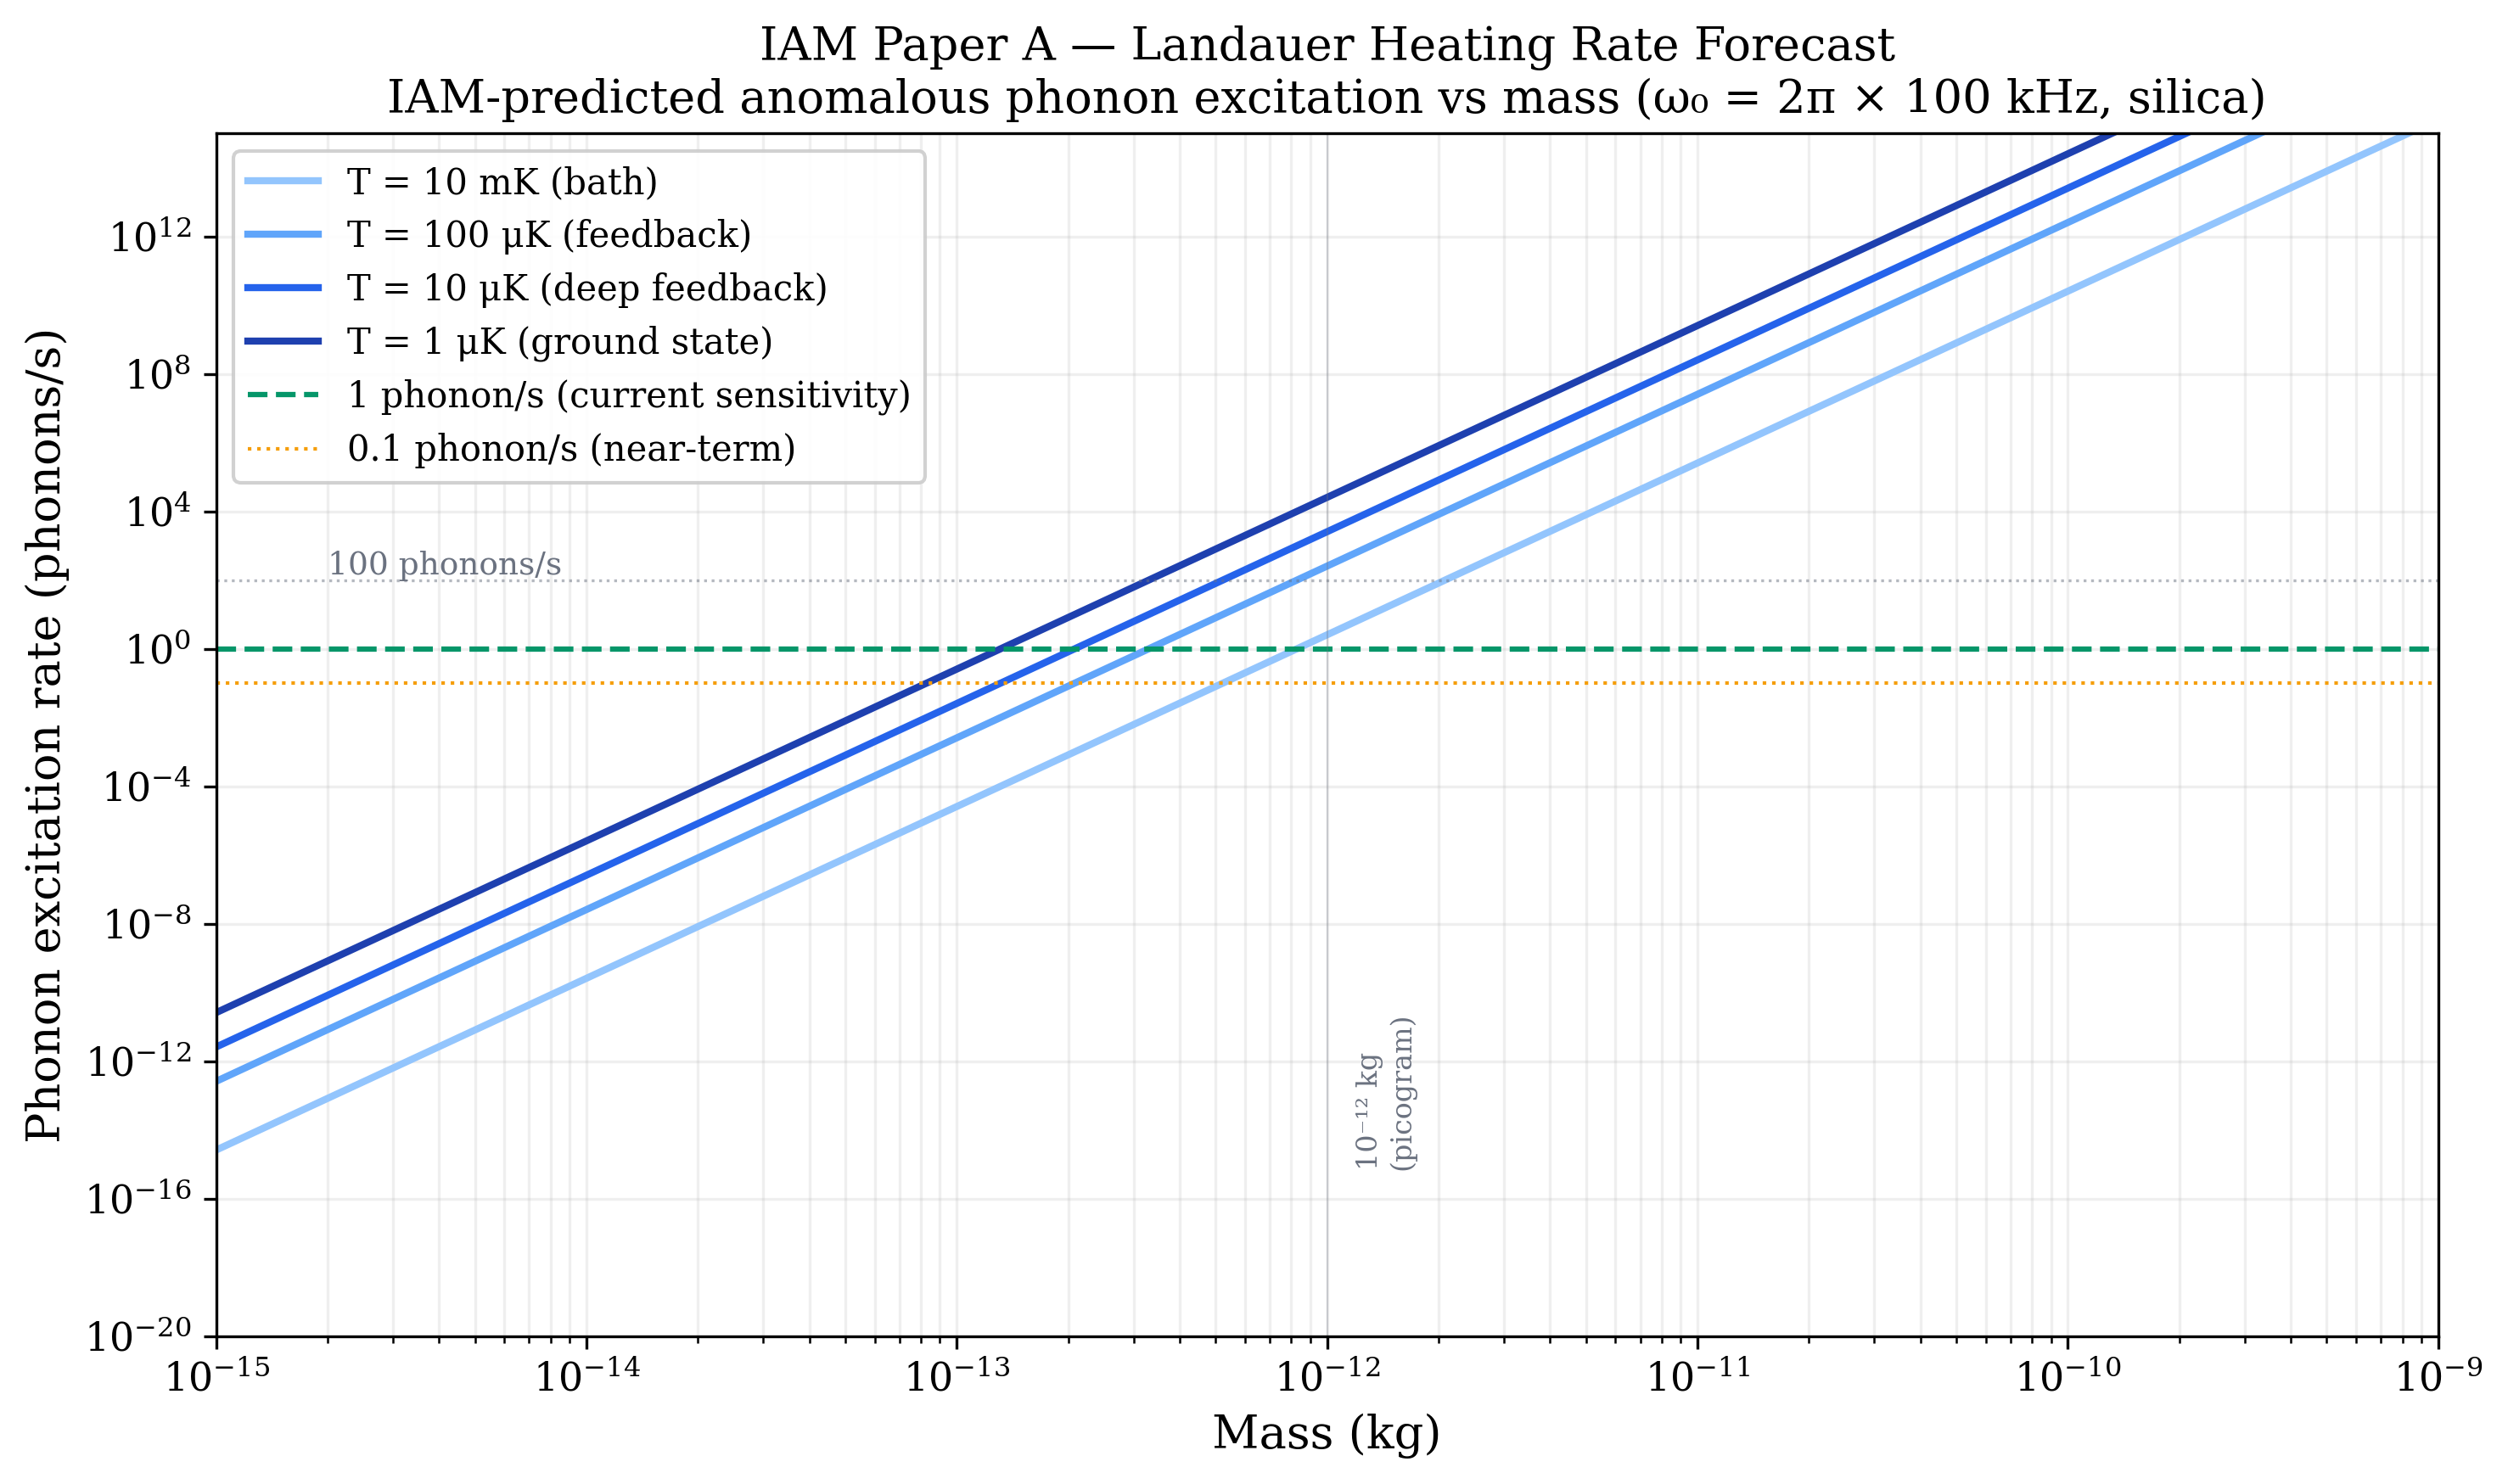
\includegraphics[width=0.85\textwidth]{fig8_phonon_heating_forecast.png}
\caption{IAM-predicted anomalous phonon excitation rate $dn/dt$ versus
mass at four temperatures ($\omega_0 = 2\pi \times 100$~kHz, silica).
Green dashed line: current optomechanical sensitivity ($\sim$1~phonon/s).
The signal is already above threshold at picogram masses at bath
temperature. Colder systems produce stronger signals ($P \propto 1/T$),
the inverse of environmental noise. This signature cannot be mimicked by
thermal or vibrational noise.}
\label{fig:phonon_forecast}
\end{figure}

\subsection{Timeline to Detection}

Figure~\ref{fig:timeline} shows the projected experimental mass trajectory
versus \IAM{} detection thresholds. Based on the field's trajectory
($\sim$10$\times$ mass increase every 3--5 years from current $10^{-19}$~kg):
\begin{itemize}
    \item \textit{Optimistic:} $3\sigma$ detection by $\sim$2028--2030,
    $5\sigma$ discovery by $\sim$2030--2032.
    \item \textit{Conservative:} $3\sigma$ detection by $\sim$2033--2035,
    $5\sigma$ discovery by $\sim$2035--2037.
\end{itemize}
This is the same timescale as Euclid testing \IAM's cosmological prediction
($\mu_0 = -0.135$ at $\sigma(\mu_0) \sim 0.04$, giving $3.4\sigma$
detection significance). Both the quantum and cosmological tests converge
in the early 2030s.

\begin{figure}[H]
\centering
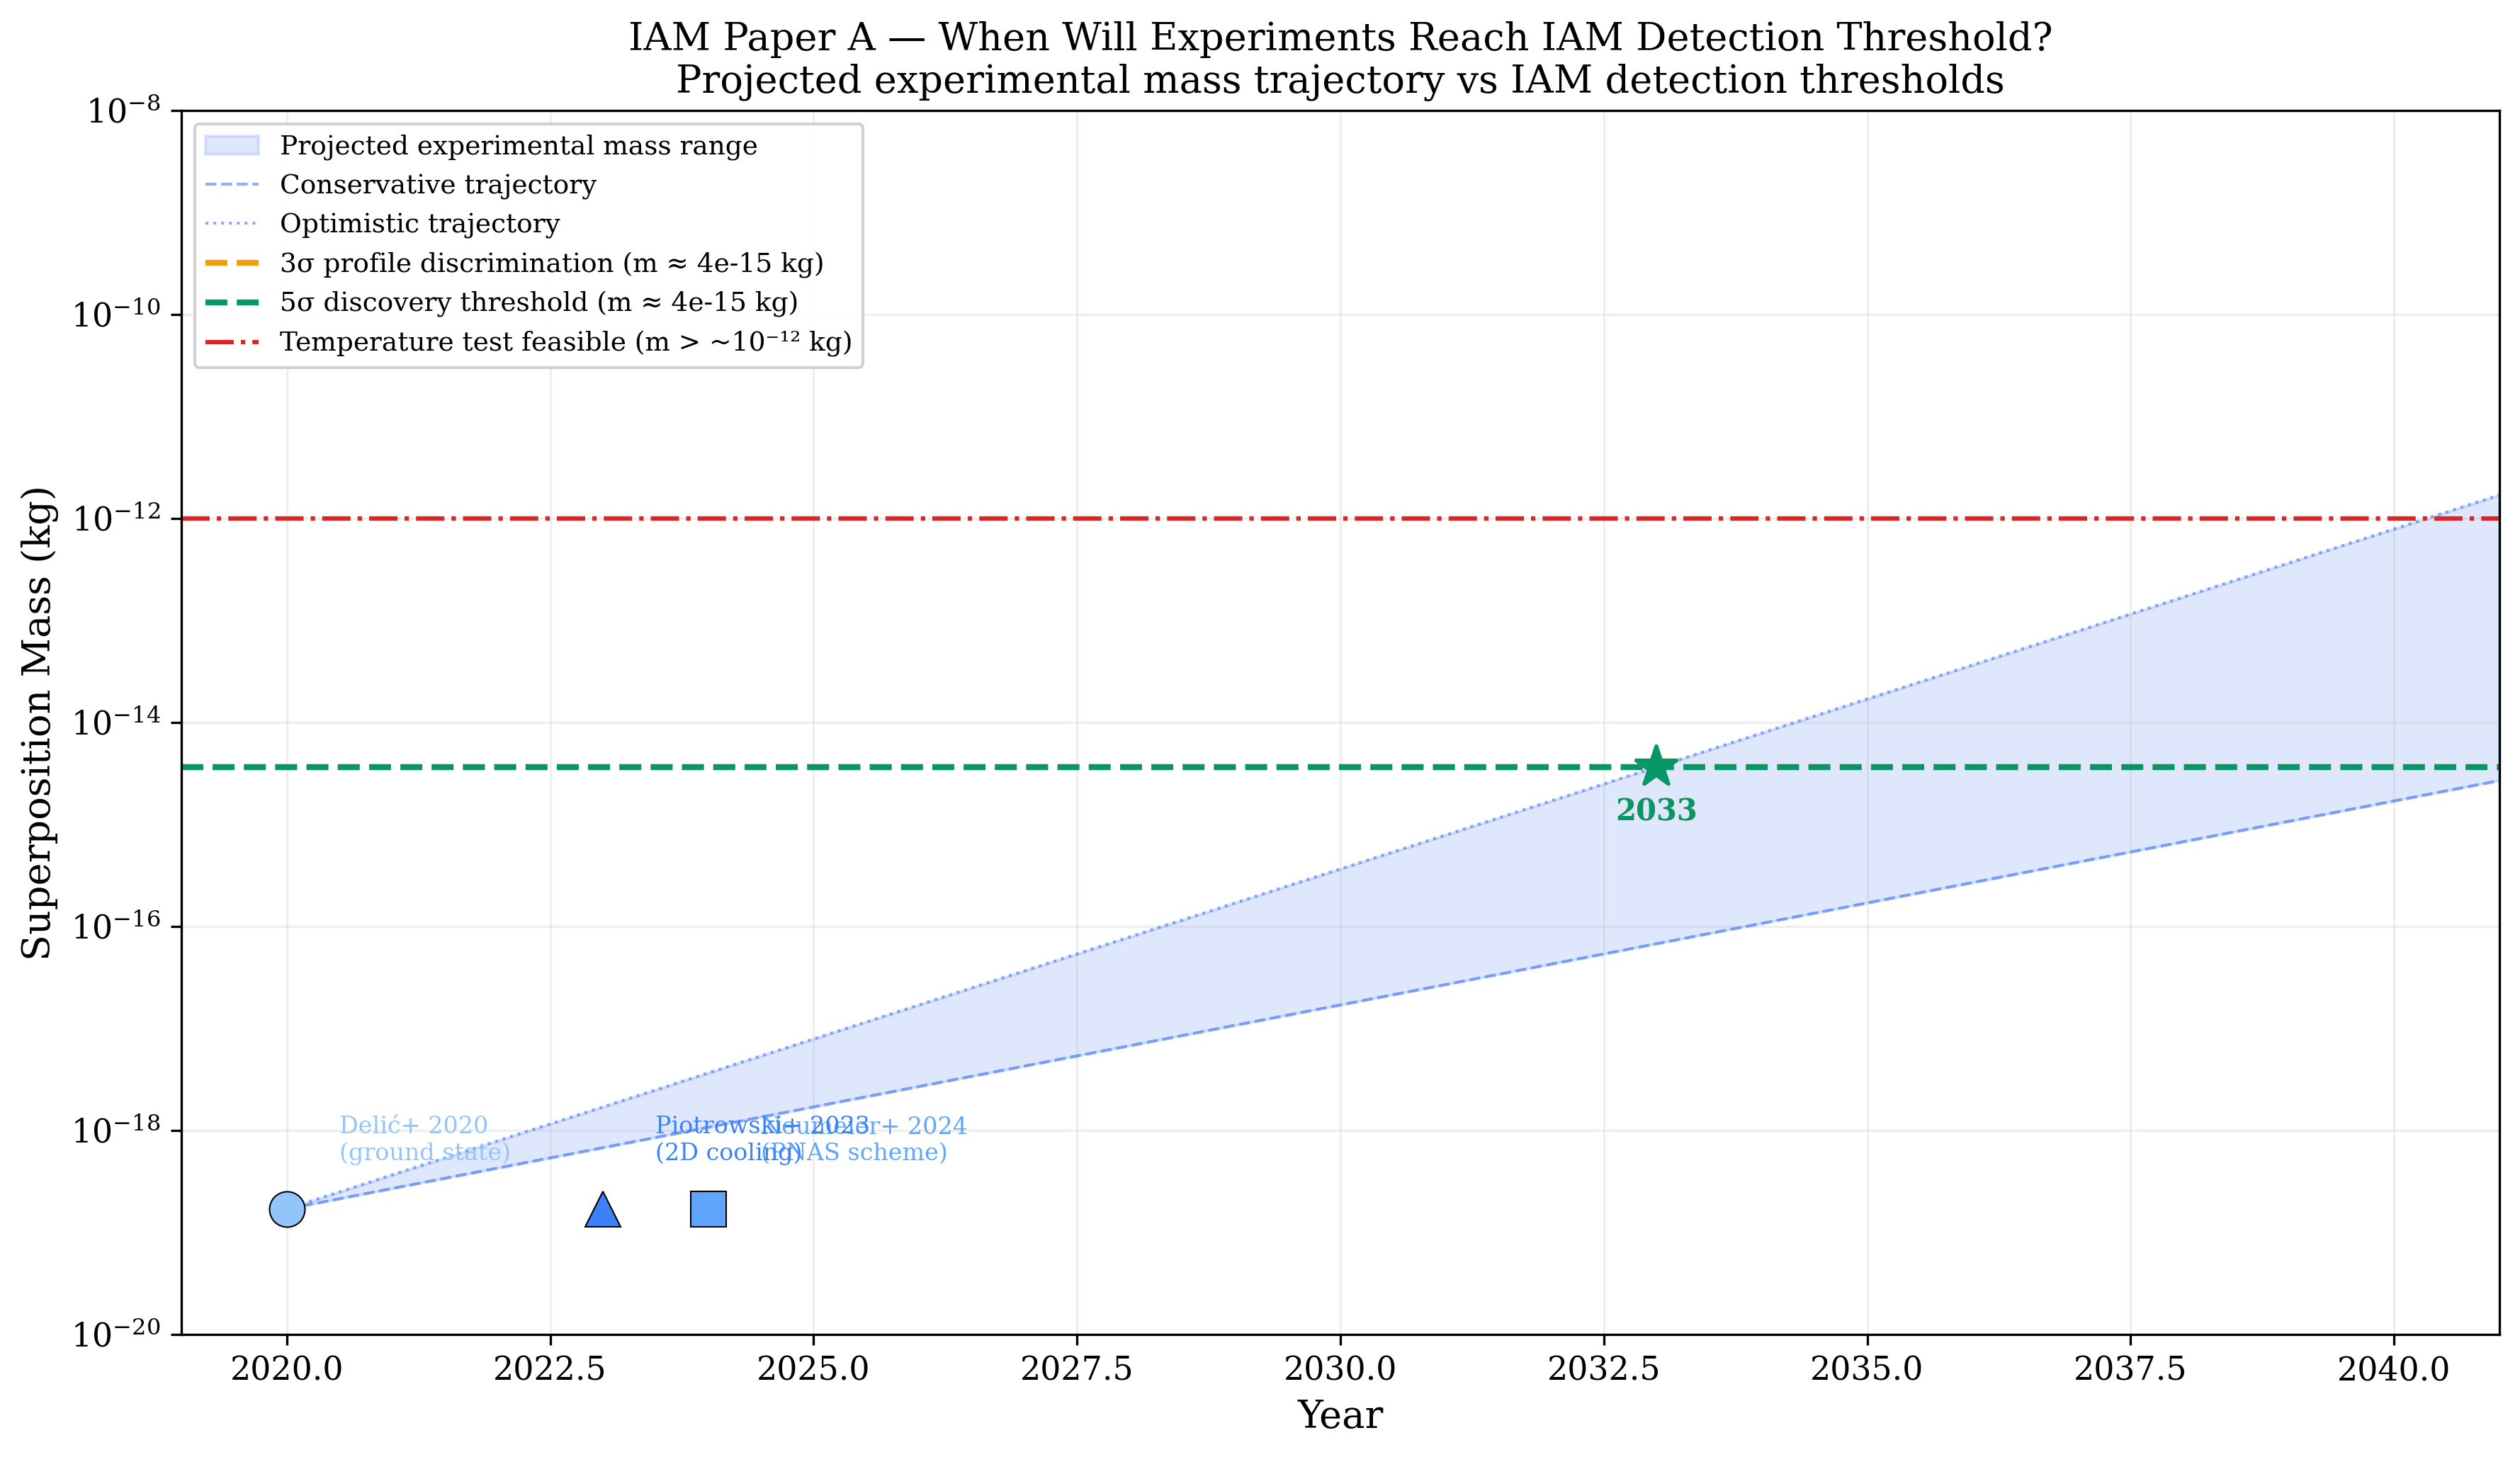
\includegraphics[width=0.90\textwidth]{fig9_timeline_forecast.png}
\caption{Projected experimental superposition mass trajectory versus \IAM{}
detection thresholds. Blue shaded band: conservative (10$\times$/5~yr)
to optimistic (10$\times$/3~yr) mass trajectories from current
$\sim$10$^{-19}$~kg. Amber/green horizontal lines: 3$\sigma$/5$\sigma$
detection thresholds from profile discrimination. Stars mark projected
crossing years. Current experiments (circles, squares, triangles) are
labeled. The optimistic trajectory reaches $5\sigma$ discovery by
$\sim$2030, converging with Euclid's cosmological test.}
\label{fig:timeline}
\end{figure}

% ============================================================
\section{Comparison with Competing Models}
% ============================================================

Table~\ref{tab:models} compares \IAM{} experimental signatures against
principal competing decoherence models. \IAM{} is uniquely identified
by all four discriminators simultaneously.

\begin{table}[H]
\centering
\caption{Comparison of decoherence models. \IAM{} is uniquely identified
by the combination of ramp profile + $T^2$ scaling + $m^{-6}$ scaling +
inverse-temperature heating. Semiclassical gravity shares $T^2$ and $1/T$
heating but differs in mass scaling.}
\label{tab:models}
\begin{tabular}{lllll}
\toprule
Model & Profile & $T$ scaling & Mass scaling & Heating \\
\midrule
\IAM{}              & $E_q$ ramp   & $T^2$    & $m^{-6}$   & $P \propto 1/T$ \\
Penrose--Di\'{o}si  & Exponential  & None     & $m^{-5/3}$ & None \\
CSL                 & Exponential  & None     & $m^{-1}$   & $P \propto T$ \\
Graviton emission   & Exponential  & $T^5$    & Various    & $P \propto T^5$ \\
Semiclassical grav. & Exponential  & $T^2$    & $m^{-2}$   & $P \propto 1/T$ \\
\bottomrule
\end{tabular}
\end{table}

% ============================================================
\section{Implications for Quantum Computing}
% ============================================================

\subsection{Current Architectures and the Gravitational Floor}

Gravitational decoherence is irrelevant for all current quantum computing
platforms. Superconducting qubits ($\sim 10^{-20}$~kg), trapped ions
($\sim 10^{-25}$~kg), and photonic systems ($\EG = 0$) all have $\tauIAM$
far exceeding any practical timescale. \IAM{} does not predict that current
quantum computers will fail.

However, \IAM{} identifies a fundamental engineering target distinct from
isolation. The \emph{isolation paradigm}: decoherence = noise $\to$ engineer
silence $\to$ move to the Moon. The \emph{\IAM{} paradigm}: decoherence =
irreversible information production $\to$ engineer reversibility $\to$
design better gates on Earth. As environmental isolation improves, residual
decoherence will increasingly be dominated by irreversible thermodynamic
interactions in gate operations. At that point, further isolation provides
diminishing returns.

\subsection{Five Principles for \IAM-Informed Quantum Computing}

\textbf{Principle 1 --- Work with the ramp.} Design computations that
complete within $t < 0.5\,\tauIAM$, where the decoherence rate is near zero.

\textbf{Principle 2 --- Minimize irreversible interaction.} Only irreversible
interactions ($Q \geq \kB T \ln 2$) advance $E_q$. Reversible interactions
do not contribute to gravitational decoherence.

\textbf{Principle 3 --- The $\Sigma = 1$ principle.} Photons have $\EG = 0$
and $\tauIAM = \infty$. Photonic qubits are fundamentally immune to
gravitational decoherence by the causal structure of spacetime, not
engineering.

\textbf{Principle 4 --- The feedback loop as resource.} When a qubit
decoheres, information is encoded rather than destroyed. Instrumenting the
environment to capture this encoding enables computation through controlled
decoherence.

\textbf{Principle 5 --- The Landauer floor as constraint.} Minimum energy
cost per irreversible operation is $\kB T \ln 2$. Optimize to operate as
close to this floor as possible.

% ============================================================
\section{Falsification Criteria}
% ============================================================

\IAM's quantum-scale predictions are falsified if:

\begin{enumerate}
\item No gravitational decoherence is detected at $10^{13}$--$10^{14}$~amu
with environmental decoherence controlled below the \IAM-predicted rate.

\item The mass scaling exponent is inconsistent with $\alpha = 6$ (\IAM)
or $5/3$ (Penrose--Di\'{o}si).

\item Temperature dependence is inconsistent with $T^2$.

\item The decoherence profile is exponential, not $E_q$ ramp.

\item Coherence times exceed $\tauIAM$ for a given mass.
\end{enumerate}

\noindent Falsification of the quantum predictions would not automatically
falsify the cosmological predictions ($\mu < 1$, $\Sigma = 1$), which could
arise from a different microscopic mechanism with the same macroscopic
consequences. The two test regimes are complementary: cosmology tests the
cumulative effect; the laboratory tests the underlying cause.

% ============================================================
\section{Connection to Cosmological Validation}
% ============================================================

The decoherence rate $\EG^3/(\hbar \kB^2 T^2 \ln 2)$ at laboratory scales
is the same physical process that, accumulated over $\sim 10^{11}$ galaxies
and 13.8~Gyr, produces the informational entropy that modifies cosmic
expansion. The laboratory measures the rate per event; cosmology measures
the cumulative effect.

At cosmological scales: $\Ea = \exp(1 - 1/a)$, modifying the
matter-sector perturbation equations and producing $\mu < 1$, $\Sigma = 1$.
At quantum scales: $E_q(\eta) = \exp(1 - 1/\eta)$, governing the
decoherence profile of individual mesoscopic systems. Same equation, same
thermodynamics, same physics at every scale.

Simultaneous positive results --- Euclid detecting $\mu < 1$ and
optomechanical experiments measuring the $E_q$ ramp at the predicted
$\tauIAM$ --- would close the loop from quantum decoherence to cosmic
acceleration.

% ============================================================
\section{Conclusion}
% ============================================================

We have derived the quantum analog $E_q(\eta) = \exp(1 - 1/\eta)$ of the
cosmological activation function $\Ea = \exp(1 - 1/a)$, extending \IAM{}
from cosmic to quantum scales. The \IAM{} decoherence timescale
$\tauIAM = \hbar \kB^2 T^2 \ln 2 / \EG^3$ contains zero free parameters
and produces four unique experimental signatures. Modified Lindblad
dynamics under the time-dependent $E_q$ rate show a measurable purity
difference peaking at $\eta \approx 0.23$, providing the optimal
discrimination measurement time. Detection forecasts show $5\sigma$
discrimination above $3.7 \times 10^{-15}$~kg, with the optimistic
detection timeline converging with Euclid's cosmological test in the
early 2030s.

The missing piece was always information.

% ============================================================
\section*{Acknowledgments}
% ============================================================

The author thanks the developers of CAMB, MGCAMB, and Cobaya for making
cosmological validation accessible to independent researchers. All MCMC
chains, configuration files, modified Fortran source code, and analysis
scripts are publicly archived at
\url{https://github.com/hmahaffeyges/IAM-Validation}.
DOI: \href{https://doi.org/10.17605/OSF.IO/KCZD9}{10.17605/OSF.IO/KCZD9}.

% ============================================================
\bibliographystyle{plainnat}
\begin{thebibliography}{99}

\bibitem{Mahaffey2026a}
H.~W. Mahaffey,
``Constraints on Late-Time $f\sigma_8$ Suppression from $\mu < 1$,
$\Sigma = 1$: Planck~2018 and Large-Scale Structure,''
submitted (2026).

\bibitem{Mahaffey2026repo}
H.~W. Mahaffey,
IAM Validation Repository (2026).
\url{https://github.com/hmahaffeyges/IAM-Validation}.
DOI: \href{https://doi.org/10.17605/OSF.IO/KCZD9}{10.17605/OSF.IO/KCZD9}.

\bibitem{Jacobson1995}
T.~Jacobson,
``Thermodynamics of Spacetime: The Einstein Equation of State,''
\textit{Phys.\ Rev.\ Lett.}\ \textbf{75}, 1260 (1995).

\bibitem{Penrose1996}
R.~Penrose,
``On Gravity's Role in Quantum State Reduction,''
\textit{Gen.\ Relativ.\ Gravit.}\ \textbf{28}, 581 (1996).

\bibitem{Diosi1987}
L.~Di\'{o}si,
``A Universal Master Equation for the Gravitational Violation of Quantum
Mechanics,''
\textit{Phys.\ Lett.\ A}\ \textbf{120}, 377 (1987).

\bibitem{Landauer1961}
R.~Landauer,
``Irreversibility and Heat Generation in the Computing Process,''
\textit{IBM J.\ Res.\ Dev.}\ \textbf{5}, 183 (1961).

\bibitem{Berut2012}
A.~B\'{e}rut et al.,
``Experimental Verification of Landauer's Principle Linking Information
and Thermodynamics,''
\textit{Nature}\ \textbf{483}, 187 (2012).

\bibitem{Ciampini2025}
M.~A. Ciampini et al.,
``Erasure of a Nonequilibrium Memory Beyond Landauer's Bound Using
Levitated Optomechanics,''
\textit{Phys.\ Rev.\ Research}\ \textbf{7}, 043321 (2025).

\bibitem{Rossi2025}
M.~Rossi et al.,
``Quantum Delocalization of a Levitated Nanoparticle,''
\textit{Phys.\ Rev.\ Lett.}\ \textbf{135}, 083601 (2025).

\bibitem{Delic2020}
U.~Deli\'{c} et al.,
``Cooling of a Levitated Nanoparticle to the Motional Quantum Ground State,''
\textit{Science}\ \textbf{367}, 892 (2020).

\bibitem{Neumeier2024}
L.~Neumeier et al.,
``Fast Quantum Interference of a Nanoparticle via Optical Potential Control,''
\textit{PNAS}\ \textbf{121}, e2306953121 (2024).

\bibitem{Kaltenbaek2012}
R.~Kaltenbaek et al.,
``MAQRO: Testing Quantum Physics in Space,''
\textit{Exp.\ Astron.}\ \textbf{34}, 123 (2012).

\bibitem{Blueprint2026}
arXiv:2512.02838,
``Experimental Blueprint for Distinguishing Decoherence from Objective
Collapse'' (2026).

\bibitem{Planck2018}
Planck Collaboration,
``Planck 2018 Results. VI. Cosmological Parameters,''
\textit{Astron.\ Astrophys.}\ \textbf{641}, A6 (2020).

\bibitem{Zurek2003}
W.~H. Zurek,
``Decoherence, Einselection, and the Quantum Origins of the Classical,''
\textit{Rev.\ Mod.\ Phys.}\ \textbf{75}, 715 (2003).

\end{thebibliography}

\end{document}


\section{Scaling Analysis of the Decoherence Rate}

We consider a generic double-commutator master equation of the form
\begin{equation}
\dot{\rho} = -\frac{i}{\hbar}[H,\rho]
- \Gamma [X,[X,\rho]],
\end{equation}
where $\Gamma$ represents the gravitationally induced decoherence rate
and $X$ characterizes the relevant mass-density operator.

Dimensional analysis suggests that for a mass distribution $M$
with characteristic size $R$, a gravitationally sourced rate
may scale as
\begin{equation}
\Gamma \sim \frac{G M^2}{\hbar R}.
\end{equation}

This scaling is consistent with earlier semiclassical estimates
in the Diósi--Penrose framework and ensures that decoherence
remains negligible for microscopic systems while becoming
relevant for macroscopic superpositions.

Importantly, for cosmological perturbations where $R$ is of
order the Hubble radius and $M$ corresponds to large-scale
density fluctuations, the resulting $\Gamma$ remains extremely
small in laboratory units but can integrate over cosmic
timescales to yield effective classicalization without violating
current experimental bounds.
